\documentclass[twocolumn]{aastex62}

\usepackage{natbib}
% \bibliographystyle{apj}
\bibliographystyle{unsrtnat}

\newcommand{\vdag}{(v)^\dagger}
\newcommand\aastex{AAS\TeX}
\newcommand\latex{La\TeX}

\graphicspath{{./}{figures/}}

\shorttitle{HAZKAT}
\shortauthors{Richey-Yowell et al. (2018)}

\begin{document}

\title{HAZKAT IV: The UV Evolution of K Stars}

\author{Tyler Richey-Yowell, Adam Schneider, Evgenya Shkolnik, ...}
\affil{School of Earth and Space Exploration, Arizona State University, Tempe, AZ 85281, USA}
\email{tricheyy@asu.edu}

\begin{abstract}

Compared to M dwarfs, K dwarfs (3,700 -- 5,200 K; 0.6 –- 0.9 M$_{\odot}$; conservative habitable zone 0.6 -- 1.1 AU from the star) have lower ultraviolet (UV) flux levels at the habitable zone, emit fewer flares, contract faster onto the main-sequence in time for terrestrial planet formation, and have wider habitable zones. These critical factors suggest that perhaps the highest potential for finding a likely habitable planet may be around K dwarfs. The UV radiation across the system’s evolution is one of the most important factors in determining if a planet is potentially habitable and if any biosignatures will be detectable with future space telescopes. We measured the evolution of the UV radiation of known K dwarf members of young moving groups and clusters ranging in age from 10 –- 625 Myr and field stars using archived GALEX data to determine how the near-UV and far-UV radiation change over important planet formation and evolution timescales. This is the first comprehensive study of UV evolution of K dwarfs and characterizes the UV environment of their potentially habitable planets, an extension of our HAZMAT program to HAZKAT.

\end{abstract}

\keywords{stars: stellar environments}

\section{Introduction}\label{sec:intro}

Astronomers have discovered thousands of exoplanets, with estimates for the occurrence of rocky planets in the habitable zone (HZ) around cool stars to be $\sim$20 for M dwarfs \citep{Dressing2015} and 22 for K dwarfs \citep{Petigura2013} from the Kepler mission statistics. The Transiting Exoplanet Survey Satellite (TESS) is expected to detect yet another 3,000 planetary candidates during its mission life \citep{Ricker2009, Ricker2014}. With so many new worlds, research has come to focus on what would make HZ planets in fact habitable \citep[e.g.][]{Cockell2016, Kaltenegger2017}. The struggle has been in finding a planet with the right balance of environmental factors of stellar lifetime, ultraviolet (UV) radiation, stellar winds, and HZ size. Currently, efforts for finding a potentially habitable planet lie with M dwarfs (2,400 –- 3,700K; 0.08 -- 0.45M$_{\odot}$; conservative HZ width 0.1AU, \citealt{Kopparapu2013}); over half of all known HZ planets are around M dwarfs. Rocky planets around these stars are more easily detectable than around Sun-like stars due to favorable star-planet radius ratios, mass ratios, and shorter periods \citep{Charbonneau2007}. However, these stars are the most active of all spectral types and HZ planets around them are close-in and most likely tidally locked \citep[e.g.][]{Checlair2017, Barnes2017}. Therefore, K dwarfs (3,700 –- 5,200K; 0.6 -- 0.9M$_{\odot}$; conservative HZ width 0.4AU, \citealt{Kopparapu2013}) may offer super-habitable conditions due to decreased stellar activity and more distant and wider HZs. The highest potential of finding a truly habitable planet may lie with K dwarfs.

M dwarf stellar activity evolution as determined in the near-UV (NUV) and far-UV (FUV) has been observed \citep{Shkolnik2014, Schneider2018}, yet there has been no comprehensive study of K-dwarf UV evolution. Archived photometric data from the UV Galaxy Evolution Explorer (GALEX; \citealt{Martin2004}) will fill the gap in our understanding in K dwarf activity evolution. Several studies regarding stellar evolution have already been conducted using GALEX photometry, such as identifying new members of young moving groups \citep{Shkolnik2010, Rodriguez2010, Rodriguez2013} and analyzing the evolution of activity for early-type stars \citep{Findeisen2011}.

%Activity indicators such as FUV levels can also be used to estimate other parameters, such as radial velocity (RV) jitter (Cegla et al. 2014), a limiting factor to the precise RVs needed to confirm and weigh exoplanets. This becomes important when prioritizing RV confirmation and characterization of planets for surveys such as Kepler (Cegla et al. 2014) or TESS, where hefty amounts of data are received. Currently, however, this estimate is only valid for FG stars. Therefore, work is needed to apply this relation to stars that are far more likely to host habitable exoplanets.

The implications of this work will be vital in determining the potentially super-habitability of planets orbiting K dwarfs by fully characterizing the UV spectral range that oversees the life-cycle of a planetary atmosphere.

Don't forget proxima flare paper.
\begin{deluxetable*}{c c c c c c c c}[th!]
\tablecaption{\small{Mass estimates spectral types at various ages based on \citet{Pecaut2013} and \citet{Baraffe2015}. } \label{tab:massest}}
\tablecolumns{8}
\tablewidth{0pt}
\tablehead{
\colhead{SpT} &
\colhead{TW Hya} &
\colhead{$\beta$ Pic} & 
\colhead{Tuc-Hor} & 
\colhead{AB Dor} &
\colhead{UMa} & 
\colhead{Hyades} & 
\colhead{Field} \\
\colhead{} & \colhead{10 Myr} & \colhead{24 Myr} & \colhead{45 Myr} & \colhead{149 Myr} & \colhead{300 Myr} & \colhead{625 Myr} & \colhead{5 Gyr}
}
\startdata
K0 & 1.30 & 0.98 & 0.90 & 0.93 & 0.92 & 0.92 & 0.89\\
K1 & 1.26 & 0.96 & 0.88 & 0.89 & 0.89 & 0.89 & 0.86\\
K2 & 1.20 & 0.93 & 0.86 & 0.86 & 0.86 & 0.86 & 0.83\\
K3 & 1.10 & 0.89 & 0.83 & 0.80 & 0.80 & 0.80 & 0.79\\
K4 & 0.98 & 0.83 & 0.80 & 0.75 & 0.75 & 0.75 & 0.74\\
K5 & 0.90 & 0.78 & 0.77 & 0.71 & 0.71 & 0.71 & 0.70\\
K6 & 0.78 & 0.74 & 0.72 & 0.63 & 0.65 & 0.66 & 0.65\\
K7 & 0.75 & 0.72 & 0.69 & 0.59 & 0.62 & 0.62 & 0.61\\
K8 & 0.72 & 0.71 & 0.66 & 0.57 & 0.60 & 0.60 & 0.60\\
K9 & 0.68 & 0.68 & 0.63 & 0.54 & 0.57 & 0.57 & 0.57\\
M0 & 0.59 & 0.62 & 0.60 & 0.51 & 0.56 & 0.53 & 0.53\\
M1 & 0.49 & 0.52 & 0.52 & 0.45 & 0.50 & 0.47 & 0.47
\enddata
\end{deluxetable*}

planet occurence rate valuable
dn / dspt

\section{The K dwarf Advantage}\label{sec:advantage}

The UV radiation incident on a planet is one of the most important factors in determining if that planet is potentially habitable and if any biosignatures will be detectable. UV radiation ionizes and photodissociates some of the most important molecules for the detection of life, e.g. H2O, CH4, and CO2, with potential for complete erosion \citep[e.g.][]{Kasting1993, Lichtenegger2010, Segura2010, Hu2012}. Additionally, UV radiation can impact the photochemistry of the atmospheres in the production of hazes in depleting atmospheres \citep{Zerkle2012, Arney2017}
%check which Arney
and ozone in oxidizing atmospheres \citep{Segura2003, Segura2005}, both of which drastically alter the planetary spectrum. This affects not only the composition, but also the detectability and stability of the atmospheres of these planets. For future missions such as JWST that will focus on spectra, a planet with a hazy or depleted atmosphere will not make a good target.

UV radiation can be split into three regimes: the extreme-UV (EUV), the far-UV (FUV), and the near-UV (NUV). EUV has the capability of additionally heating and inflating a planet’s upper-atmosphere, thus exacerbating and accelerating its erosion \citep{Koskinen2010, Lammer2007}. However, other than very limited data from the EUVE satellite, no information in this wavelength regime exists. These values are extremely important though, since photochemical atmospheric models of HZ planets and abundance rate models require an input of EUV stellar fluxes, currently being extrapolated from a limited number of X-ray observations. Therefore, realistic information regarding the NUV, FUV, and X-ray is of the utmost importance for using models to answer questions regarding planetary atmospheres. 

While current popularity resides among M dwarfs for the most likely to host identifiable habitable planets, excess flaring and tidal locking in the HZ is cause for concern \citep[e.g.][]{Shields2016}. However, attention to K dwarfs is now rising. Both \citet{Heller2014} and \citet{Cuntz2016} identified early and mid-K spectral types as “super-habitable worlds”, analyzing several factors to determine the “Habitable-Planetary-Real-Estate Parameter” (HabPREP): the frequency of different stars, the speed of stellar evolution, the size and timescale of the HZ, UV and X-ray emission and flare frequency and power. As seen in Figure 2, the HabPREP value is at a maximum (i.e. the highest probability of having a habitable planet) in the early-K dwarf regime. Additionally, the longer lifetimes of the continuous HZ of these types of stars compared to F and G stars allow for life to “tune” their environment and develop a more compromising biosignature; however, planets around M dwarfs may lose their atmosphere within 100Myr based on severe UV irradiance \citep{Airapetian2017}. \citet{Lingam2017} find that K6V stars around 0.67M  would take the least amount of time for complex life to develop since increased oxygen levels from UV photolysis permit the emergence of complex life, while more recent work by \citet{Arney2017}
%vheck arney
has confirmed that there is a similar “K dwarf advantage” and that a planet orbiting a K6V star has the potential to produce detectable CH4 and O2. K dwarf UV evolution is thus critical for determining planetary habitability.

\section{K Dwarf Sample}\label{sec:sample}

We consider the young moving groups and clusters in \citet{Shkolnik2014} and \citet{Schneider2018} as well as three additional associations ranging in age from 10 Myr to 625 Myr. The associations included are TW Hydra (10 Myr, \citealt{Bell2015}), Beta Pictoris (22 Myr, \citealt{Shkolnik2017}), Carina (40 Myr, \citealt{Torres2008}), Columba (45 Myr, \citealt{Zuckerman2011}), Tucana-Horologium (45 Myr, \citealt{Bell2015}), AB Doradus (149 Myr, \citealt{Bell2015}), Ursa Majoris (300 Myr, \citealt{King2005}), Praesepe (600 Myr, \citealt{Kraus2007}), and Hyades (625 Myr, \citealt{Perryman1997}), in addition to field stars (taken to be 5 Gyr).

Taking into account the wide range of ages in this study, we must consider how similar spectral types represent different masses over various ages. 

Table \ref{tab:massest}


The field stars were selected by doing a SIMBAD search for main sequence K stars within 25pc that were not close binaries or known members of associations. 




We got the members from these papers:

Spectral types are different per age - K0 young is not K0 old. We went with masses 0.6 -- 0.9 M$_{\odot}$ but allowed one step lower and higher to account for spectral type uncertainty.





\section{GALEX Photometry}\label{sec:photometry}

\begin{figure*}[t]
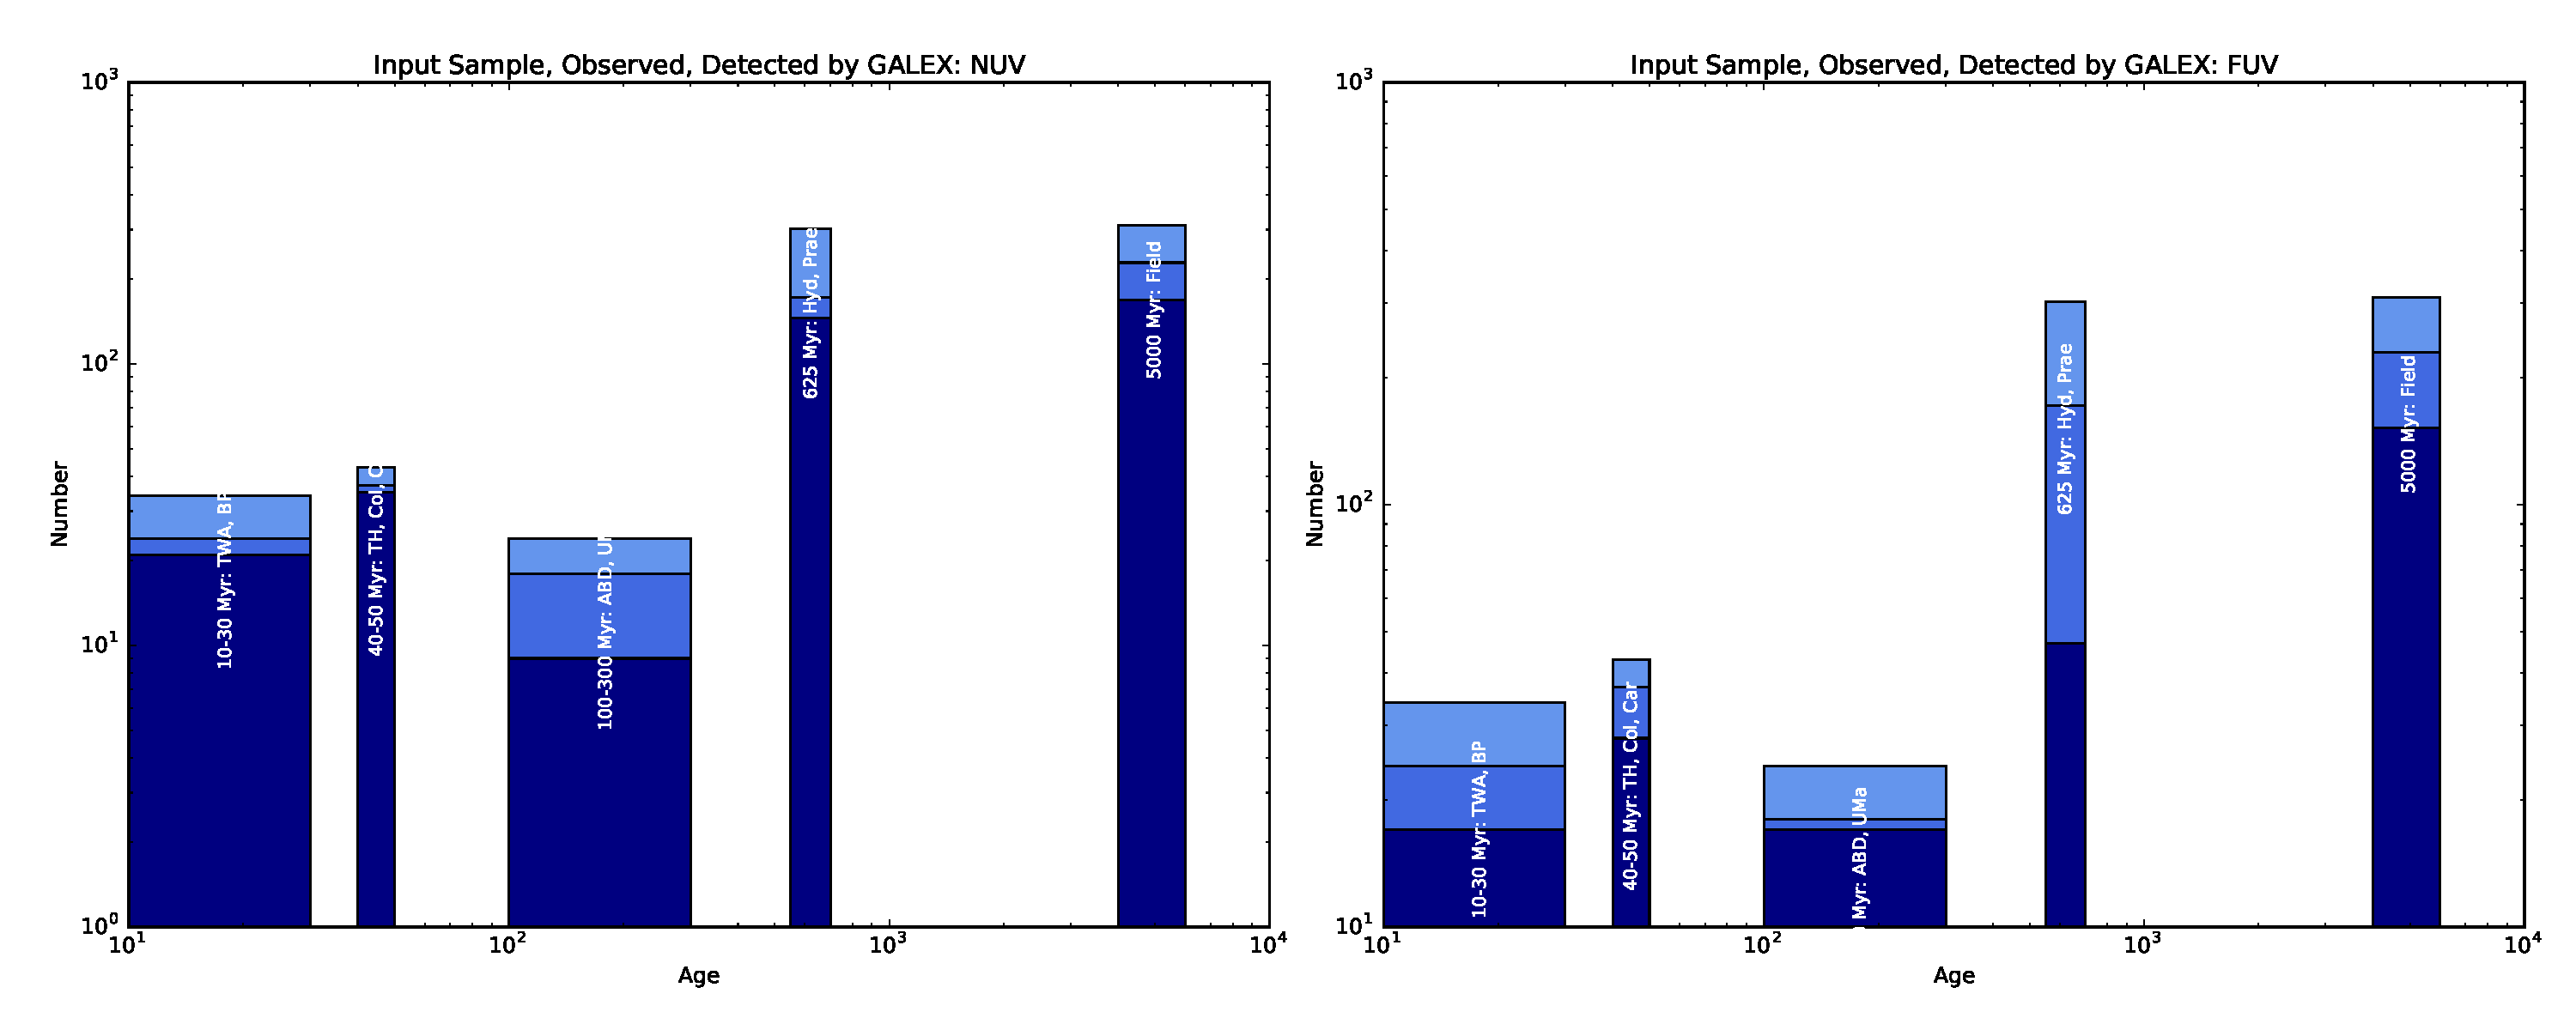
\includegraphics[width=\linewidth]{galex_observations.pdf}
\caption{Filler image for now. Need to fix scaling. \label{fig:galex_observations}}
\end{figure*}


Since GALEX ran from 2003 to 2012, we proper motion corrected our targets to the average J2007 since we did not know the observation dates beforehand. We then cross referenced our sample to GALEX using the GALEXview tool\footnote{http://galex.stsci.edu/galexview/} with a search radius of 10". [equation?] The NUV and FUV detectors go non-linear at 104 counts s$^{-1}$ and 34 counts s$^{-1}$, respectively, correlating to a magnitude of $\approx$15 for both NUV and FUV. Measured magnitudes less than 15 were thus excluded from our data. Additionally, we excluded detections with photometric flags for bright star window reflection, dichroic reflection, detector run proximity, or bright star ghost. We visually inspected the GALEX tiles for each observation to ensure that there was no contamination that was not caught by the flags. 



\begin{figure*}[h]
\centering
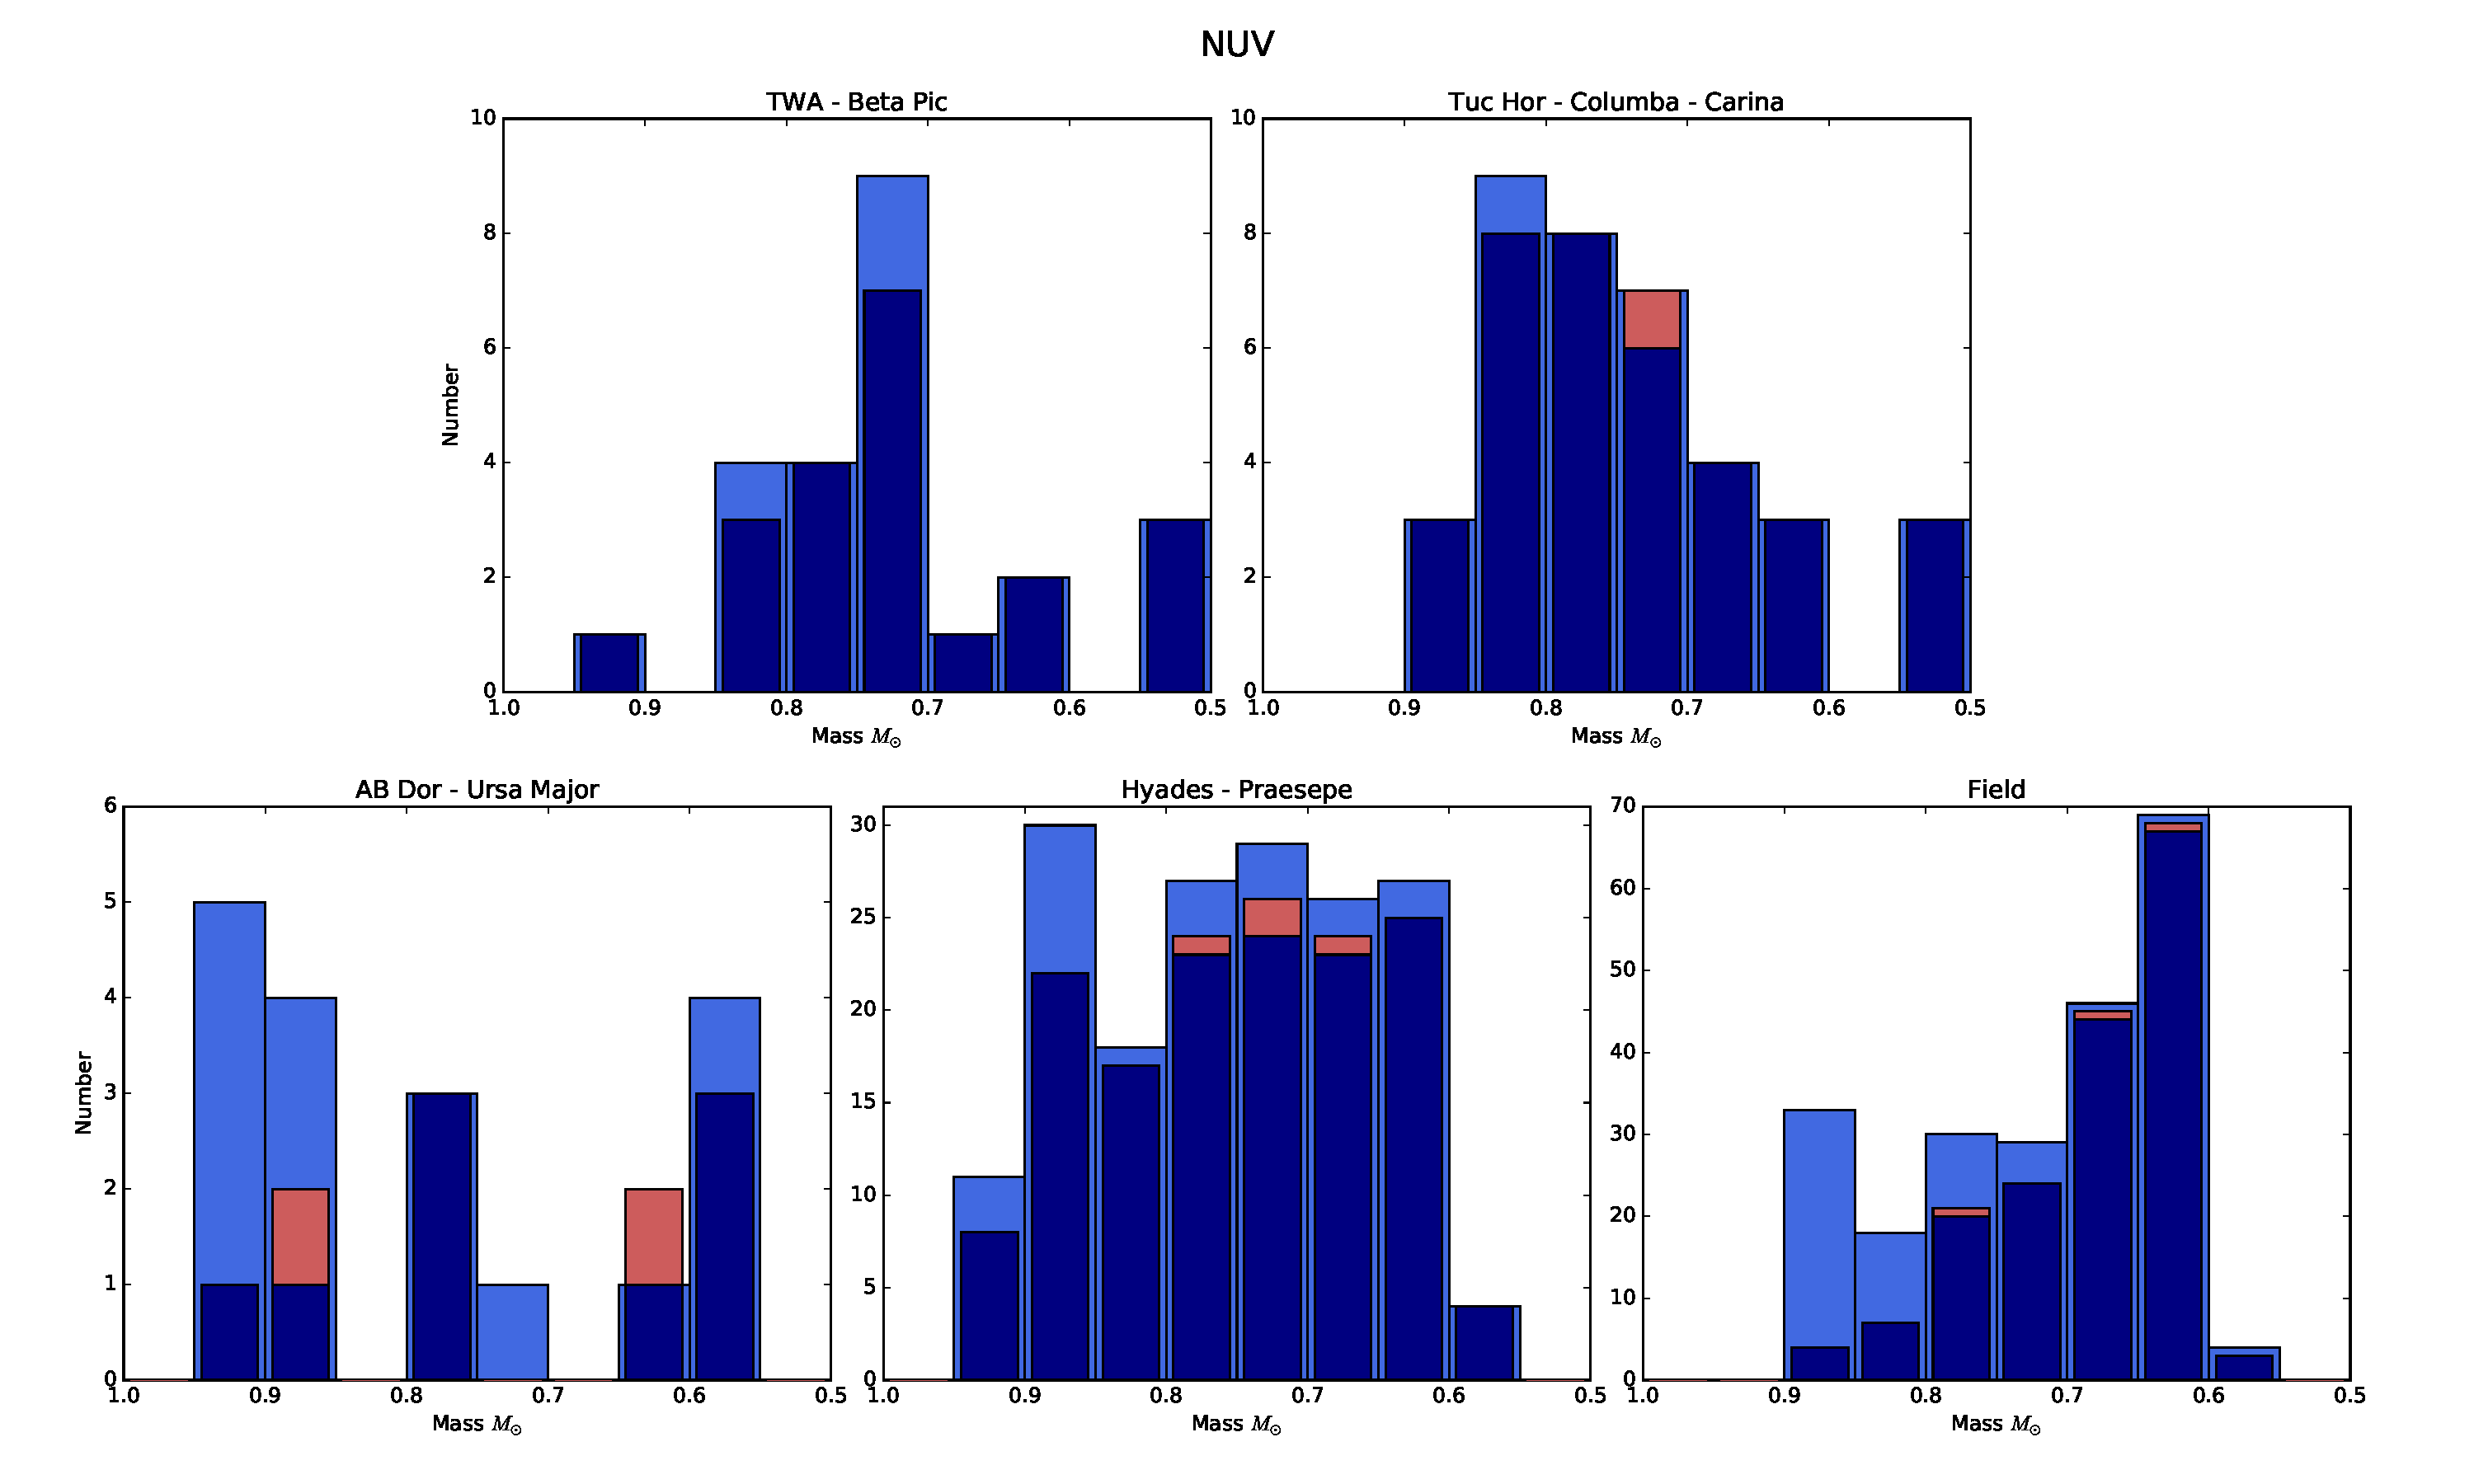
\includegraphics[width=.9\linewidth]{massdistributions_nuv.pdf}
\caption{Filler image for now. Need to fix scaling. \label{fig:massdistributions_nuv}}
\end{figure*}

\begin{figure*}[h]
\centering
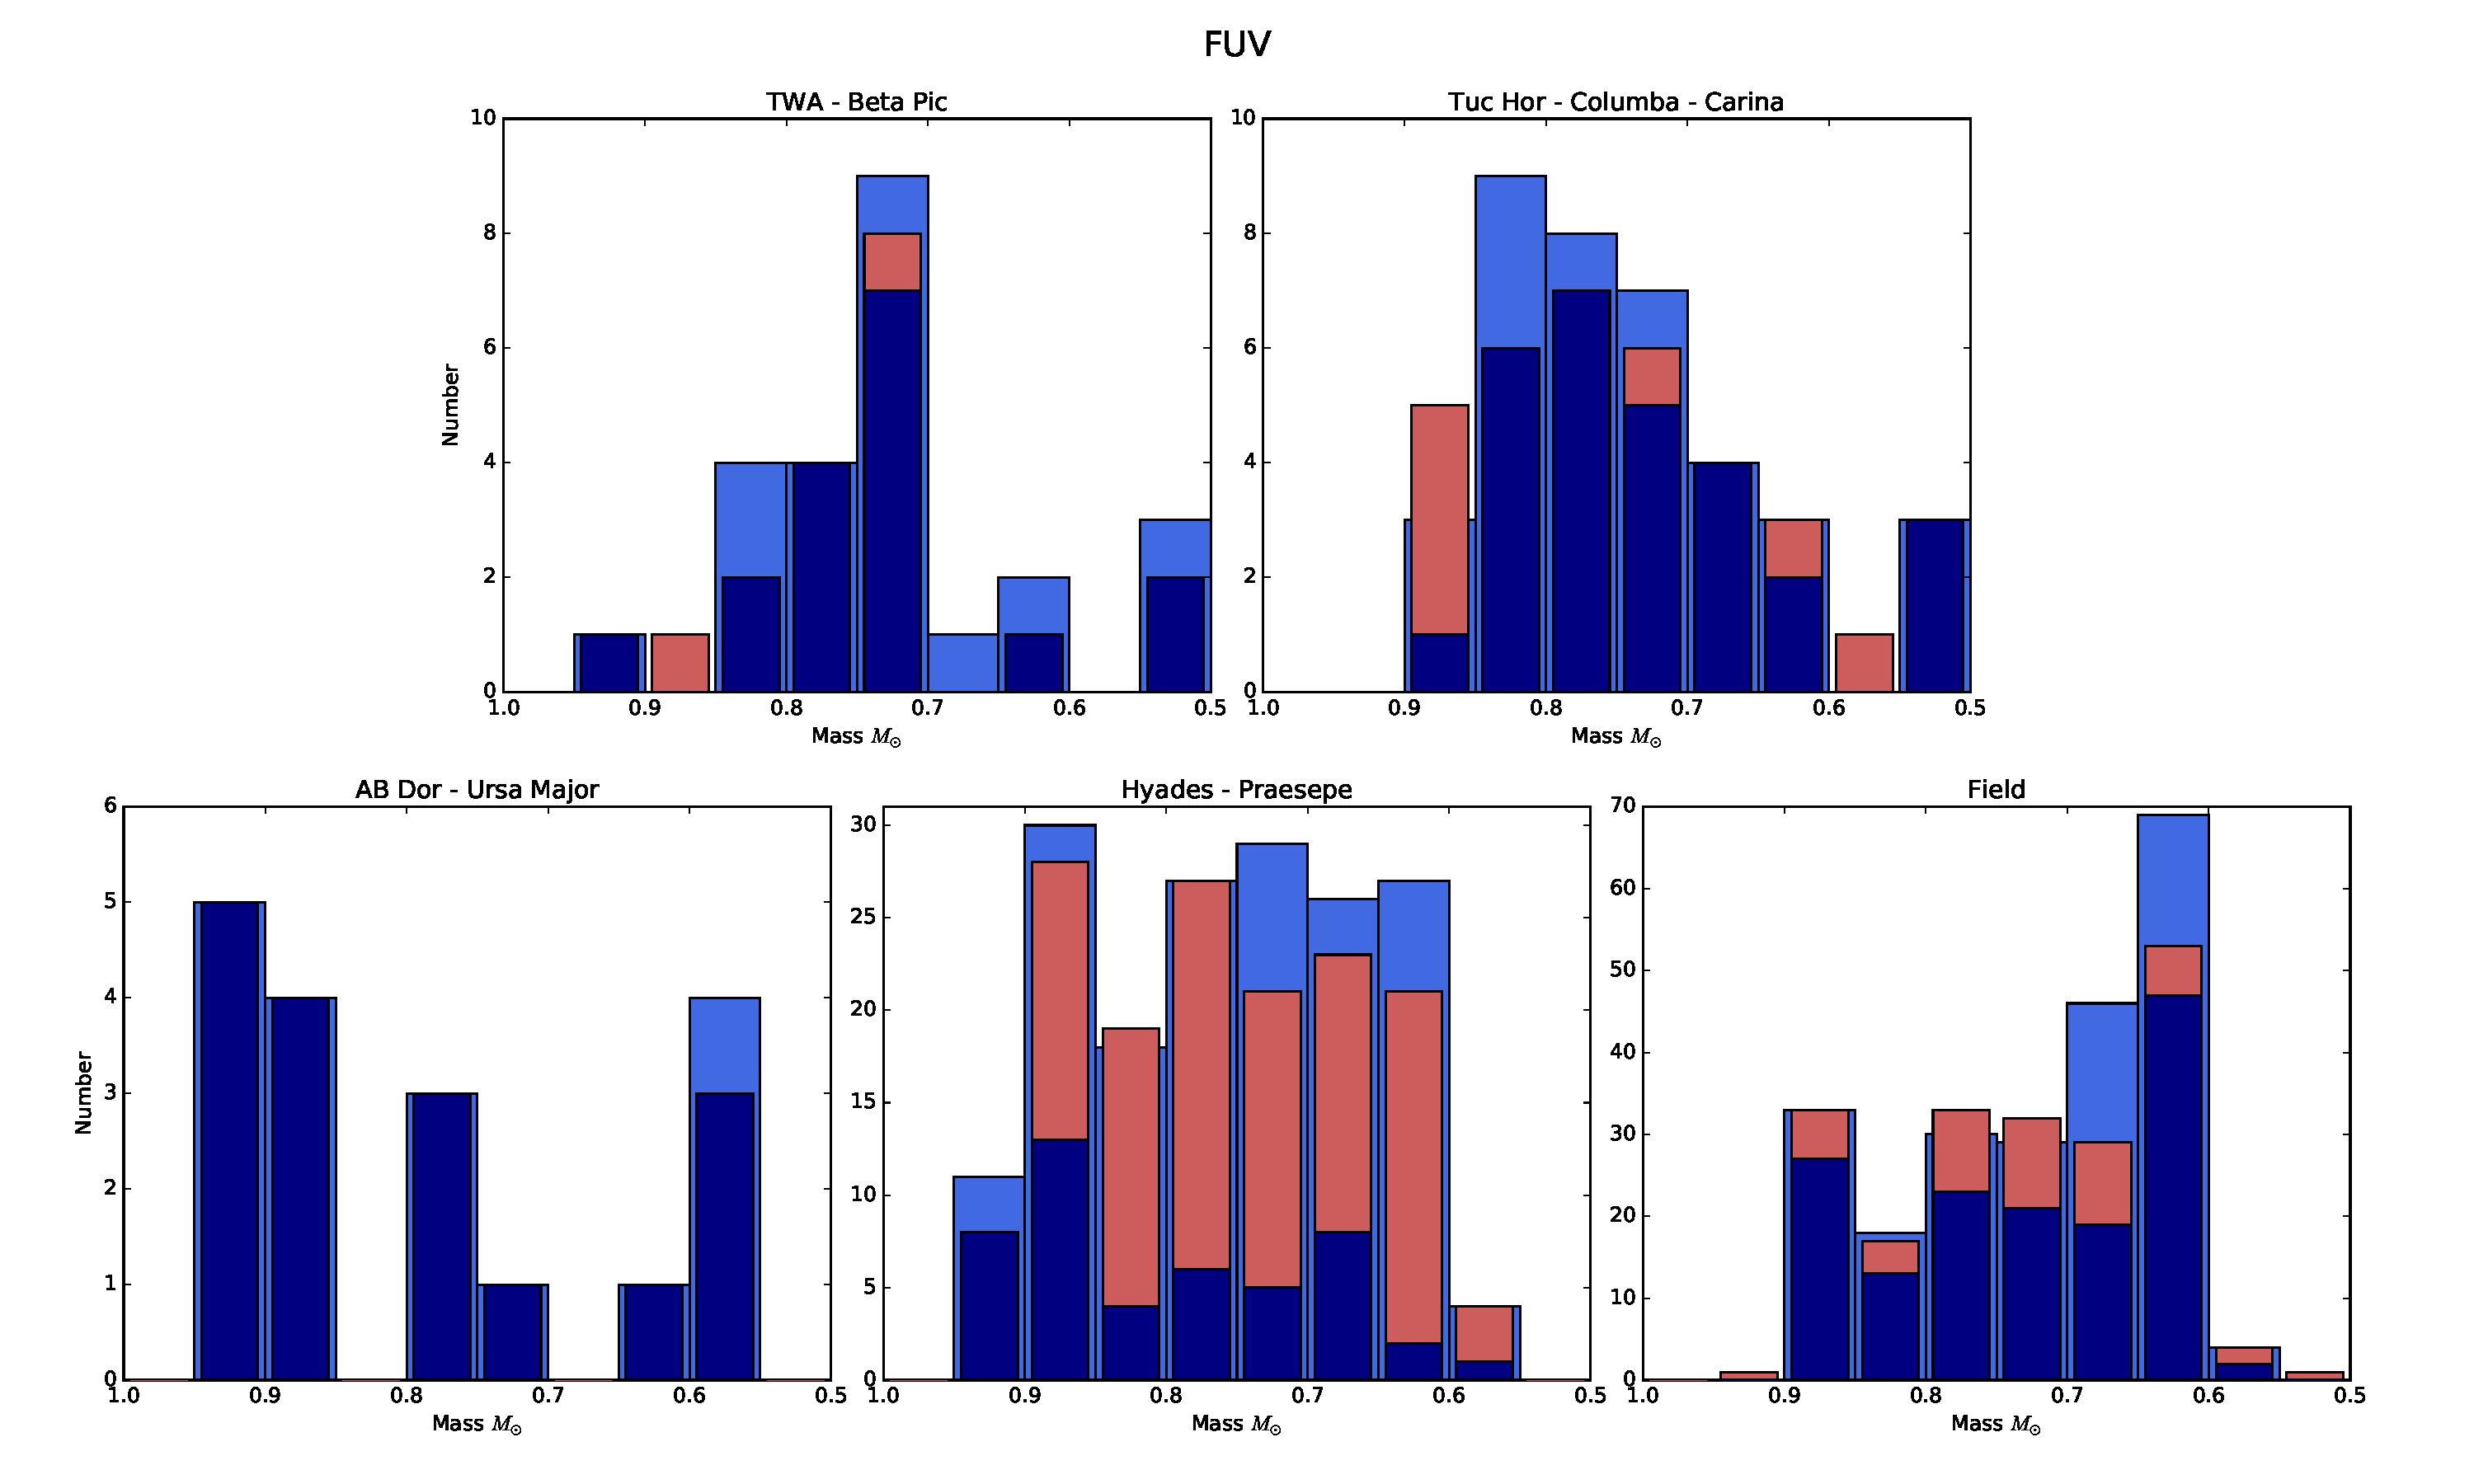
\includegraphics[width=.9\linewidth]{massdistributions_fuv.pdf}
\caption{Filler image for now. Need to fix scaling. \label{fig:massdistributions_fuv}}
\end{figure*}

\begin{figure*}[th]
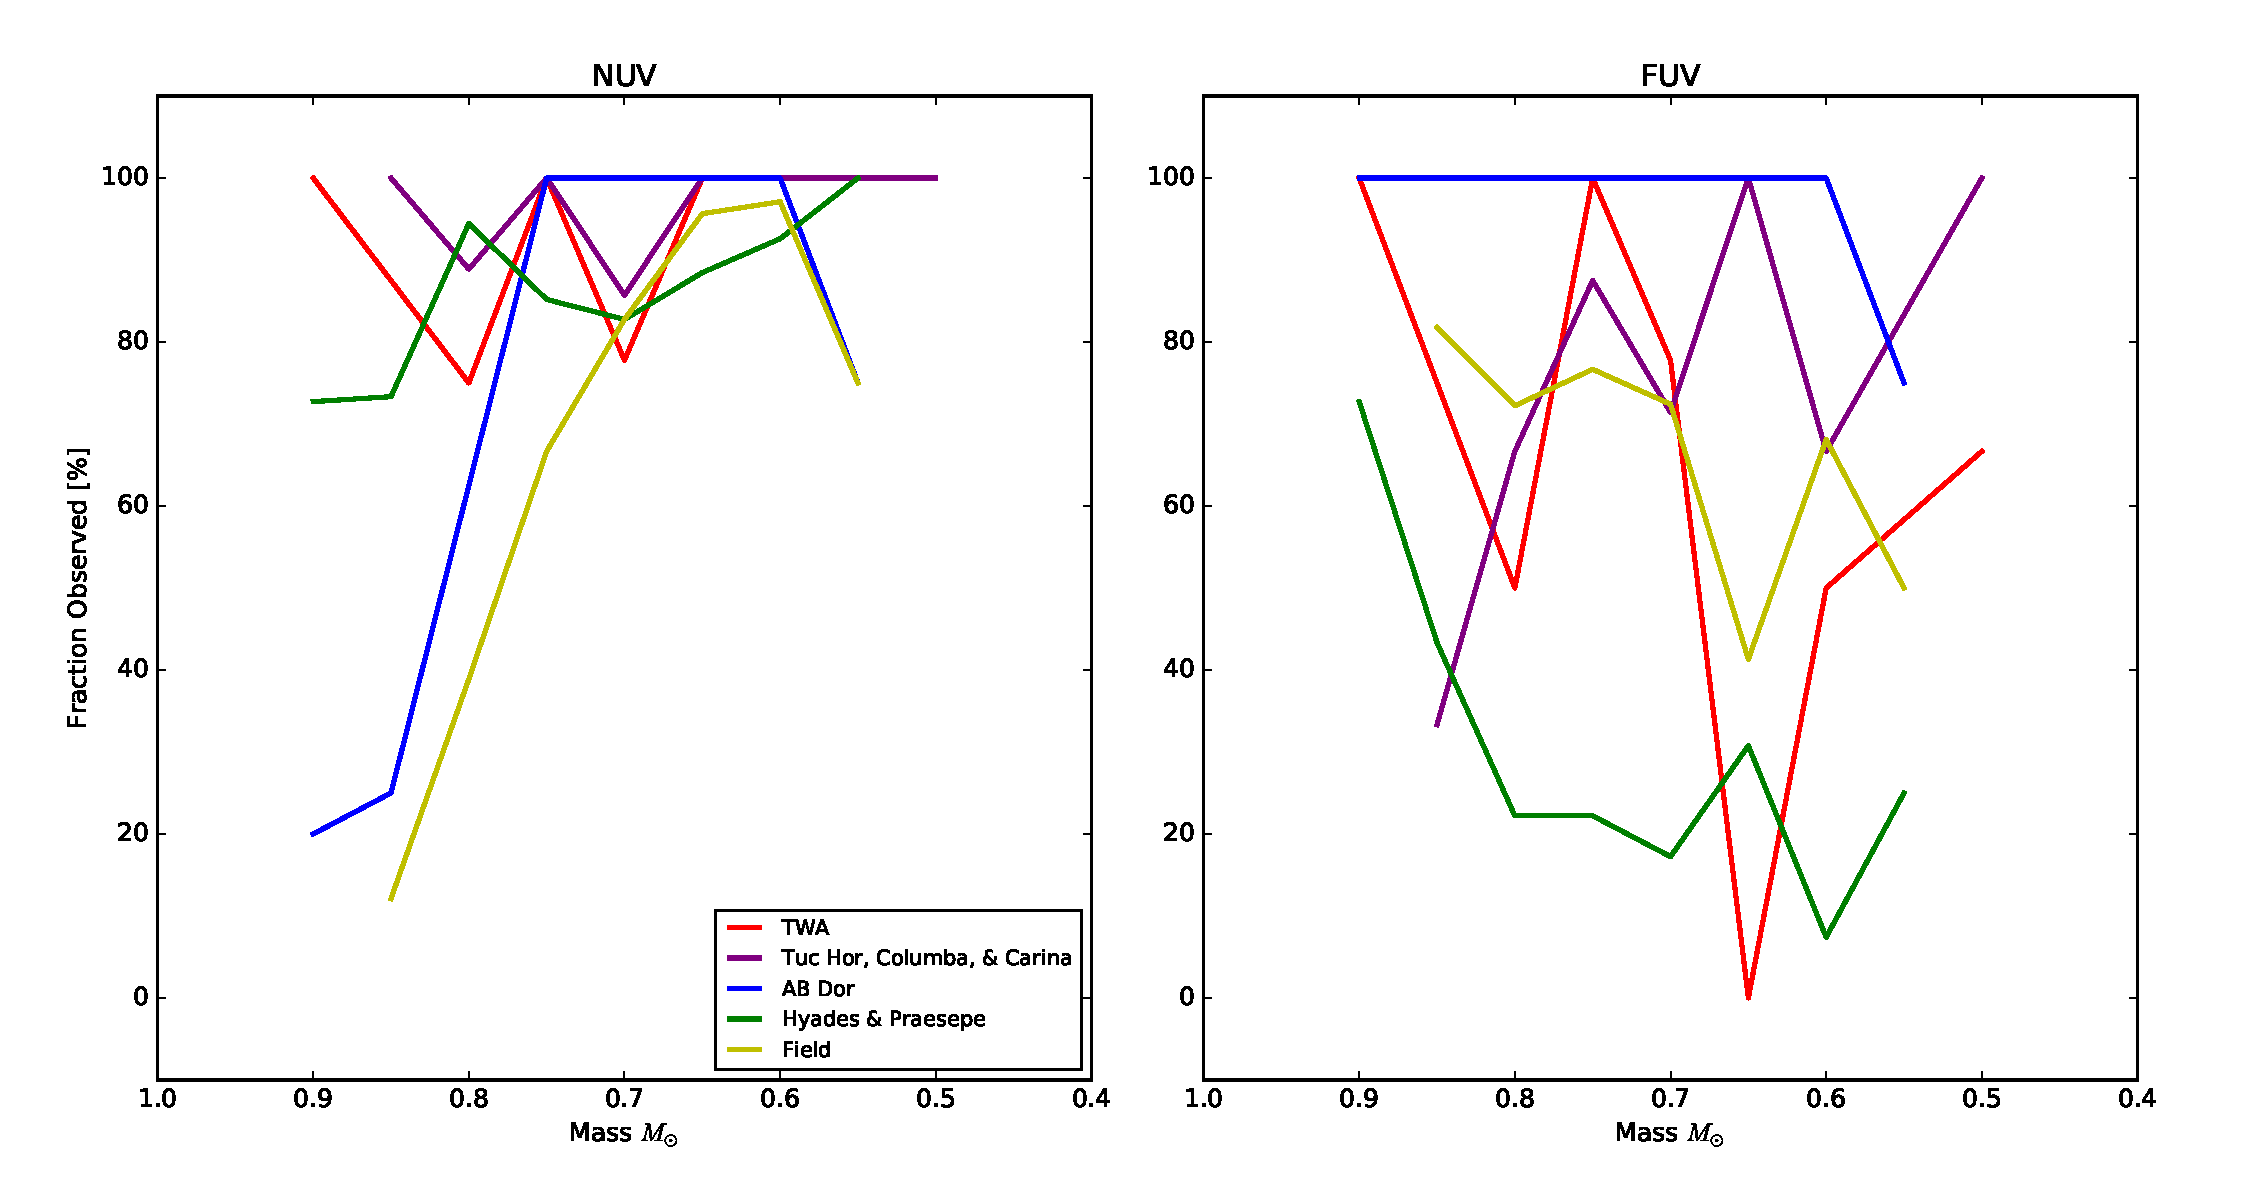
\includegraphics[width=\linewidth, height=3in]{massfractions.pdf}
\caption{Filler image for now. Need to fix scaling. \label{fig:mass_fractions}}
\end{figure*}

A comparison of the number of objects that were in our input sample, observed by GALEX, and then detected with useful photometry can be seen in Figure \ref{fig:galex_observations}. [comment on these percentages]

For some objects there were multiple observations with multiple exposure times, in which case we took the weighted mean of the magnitude as our measurement and the weighted standard deviations as our uncertainty.

Some objects were detected by GALEX but not observed. In this case, we calculated an upper limit for the object by repeating the search with a 10' search. We then limited the results to the exposure time with the most observations. [We then perform a power-law fit to the relationship between the signal-to-noise ratio (S/N) and the signal of each nearby detection, excluding those objects that exceed the saturation threshold of the detector or with photometric flags listed earlier in this section. We then take the magnitude that a source would have with a S/N of 2 using our power-law fit as an upper limit.]




\section{Evolution of the Photospheric UV Emission}

\begin{figure*}[th]
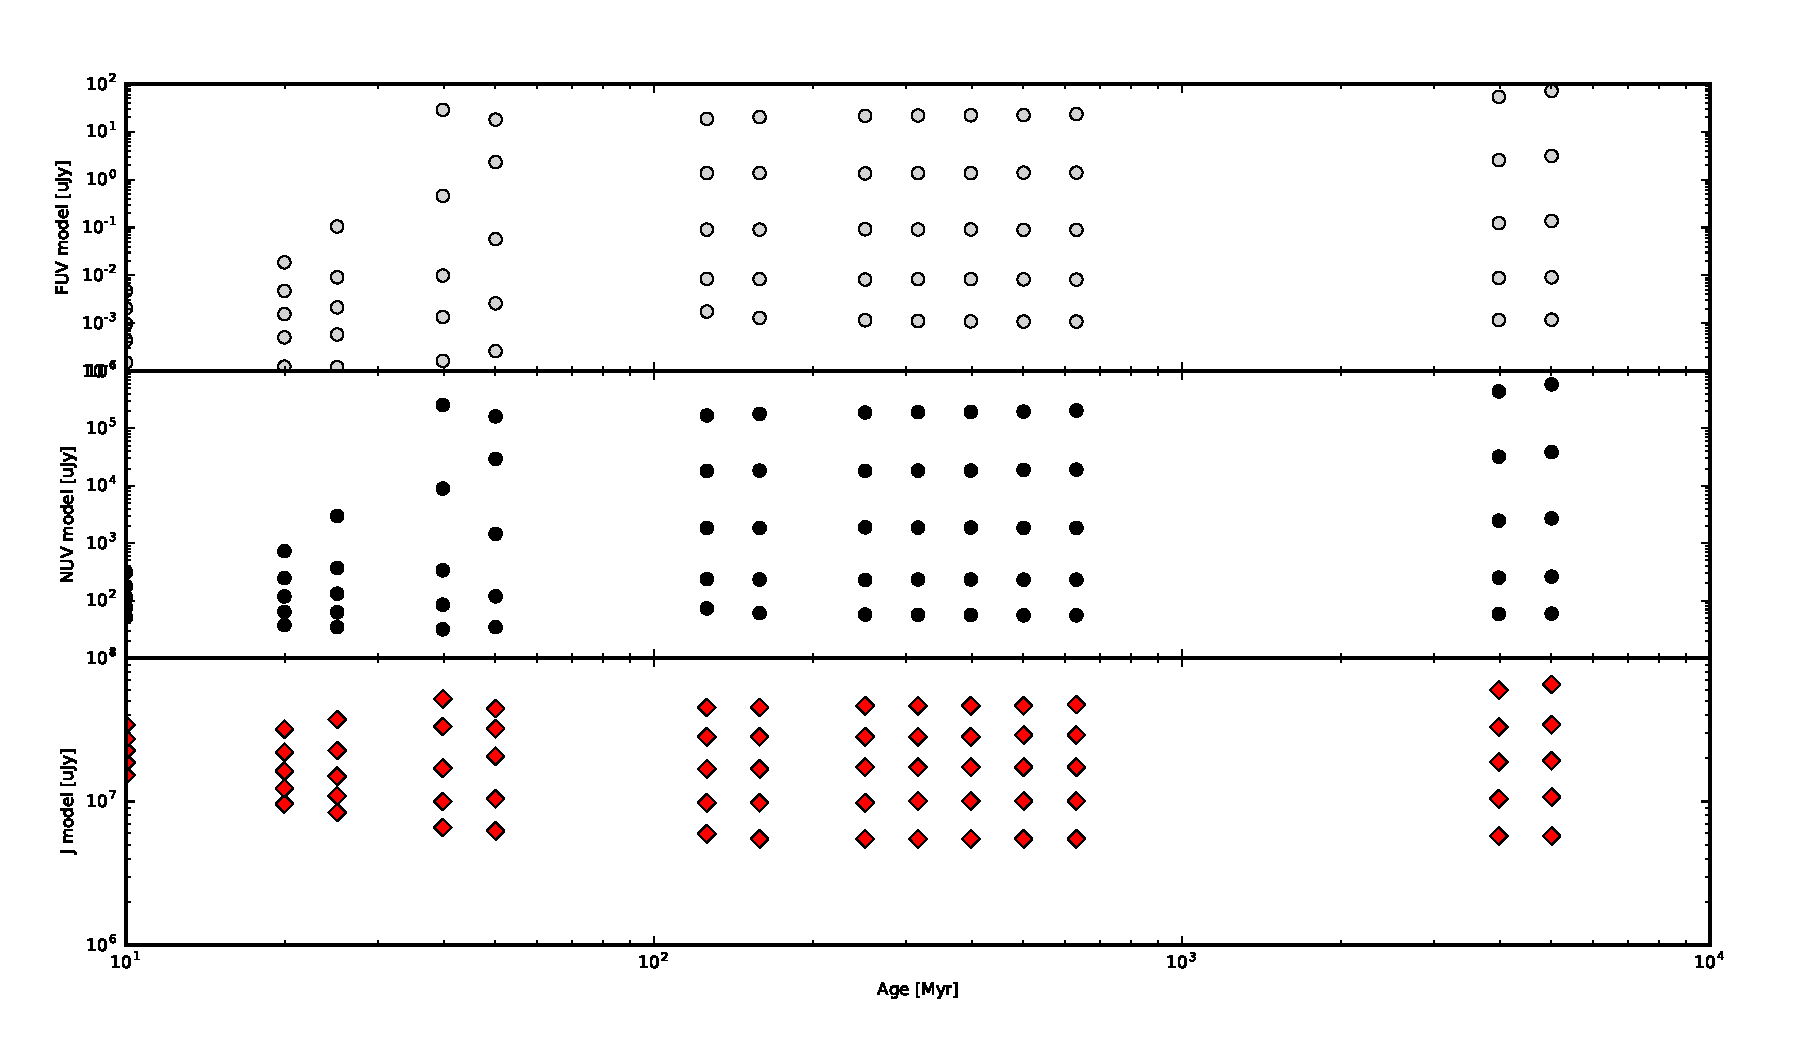
\includegraphics[width=\linewidth]{mfd_vs_age.pdf}
\caption{Filler image for now. Need to fix scaling. \label{fig:mvd_vs_age}}
\end{figure*}

\section{Results}

in section \ref{sec:photometry}

\subsection{Photospheric Contribution}

\begin{figure*}[h]
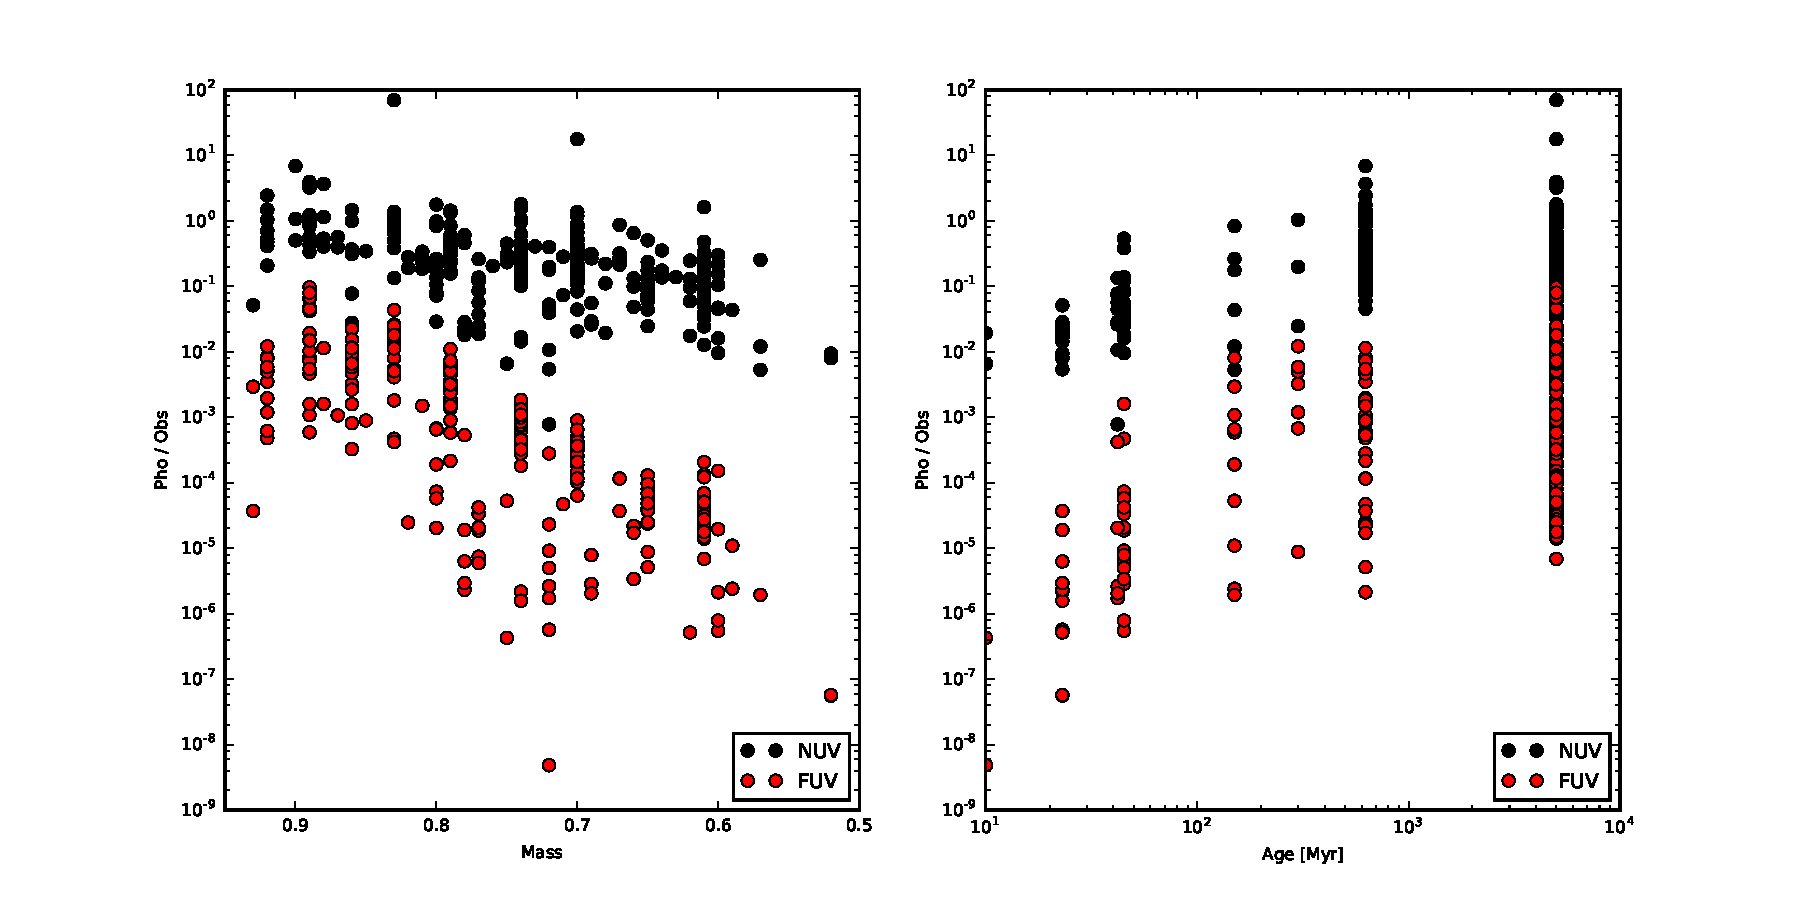
\includegraphics[width=\linewidth]{phot_obs.pdf}
\caption{Filler image for now. Need to fix scaling. \label{fig:phot_obs}}
\end{figure*}

\subsection{Evolution of the NUV and FUV Emission}

\begin{figure*}[h]
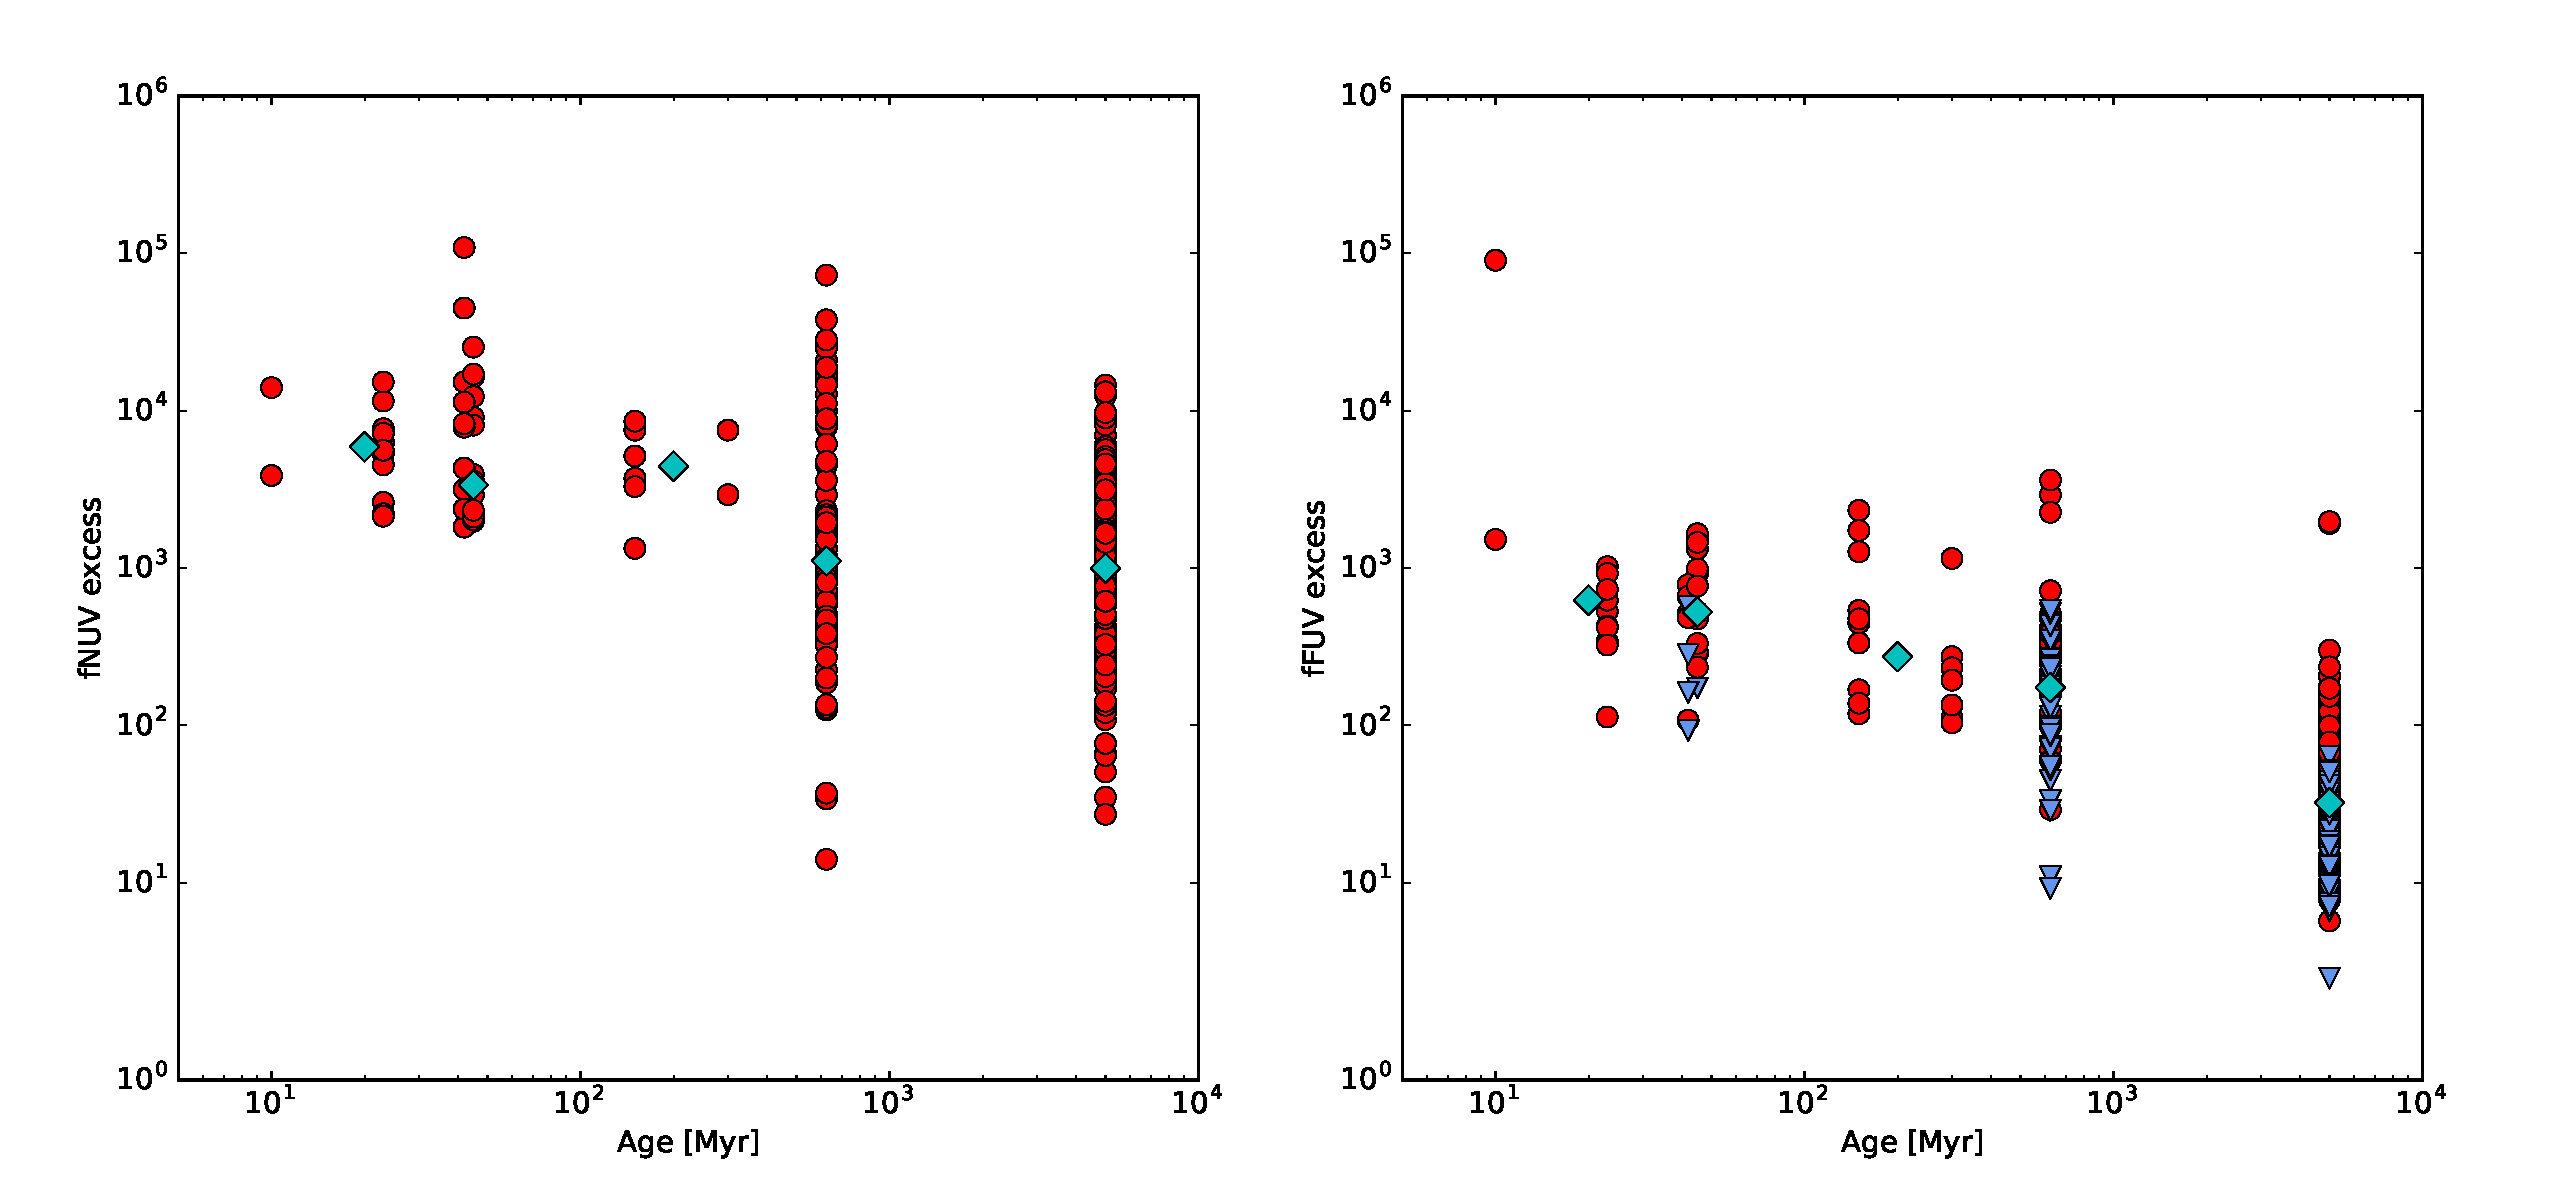
\includegraphics[width=\linewidth]{ffdensity_age_NO_J.pdf}
\caption{Filler image for now. Need to fix scaling. \label{fig:ffdensity_age}}
\end{figure*}

\begin{figure*}[h]
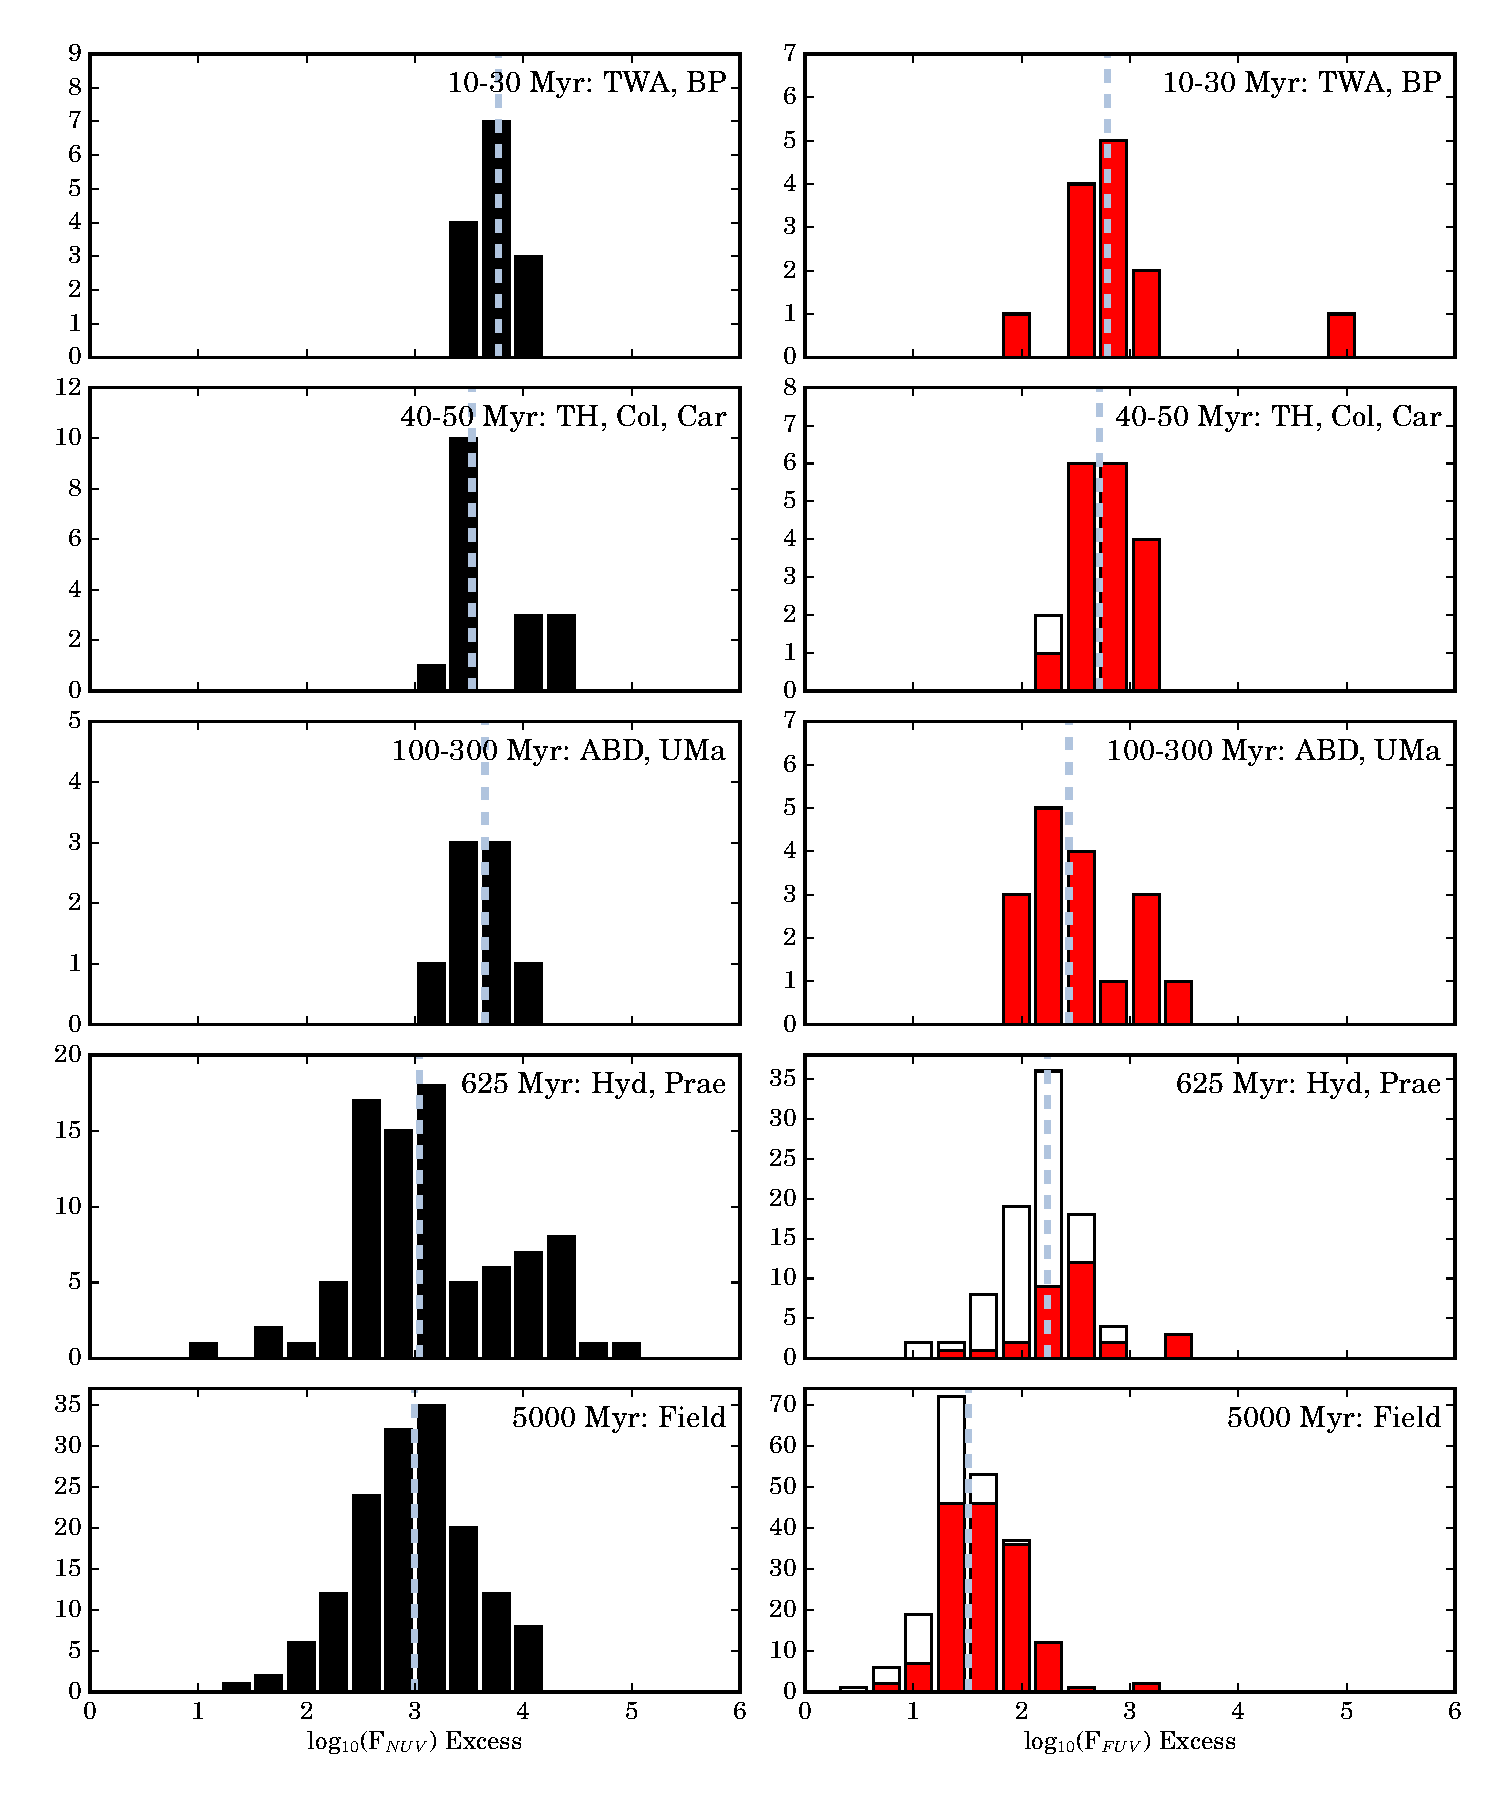
\includegraphics[width=\linewidth]{histfd_NO_J.pdf}
\caption{Filler image for now. Need to fix scaling. \label{fig:histfd}}
\end{figure*}


\subsection{The Relationship Between GALEX FUV and NUV for K Stars}

\begin{figure*}[h]
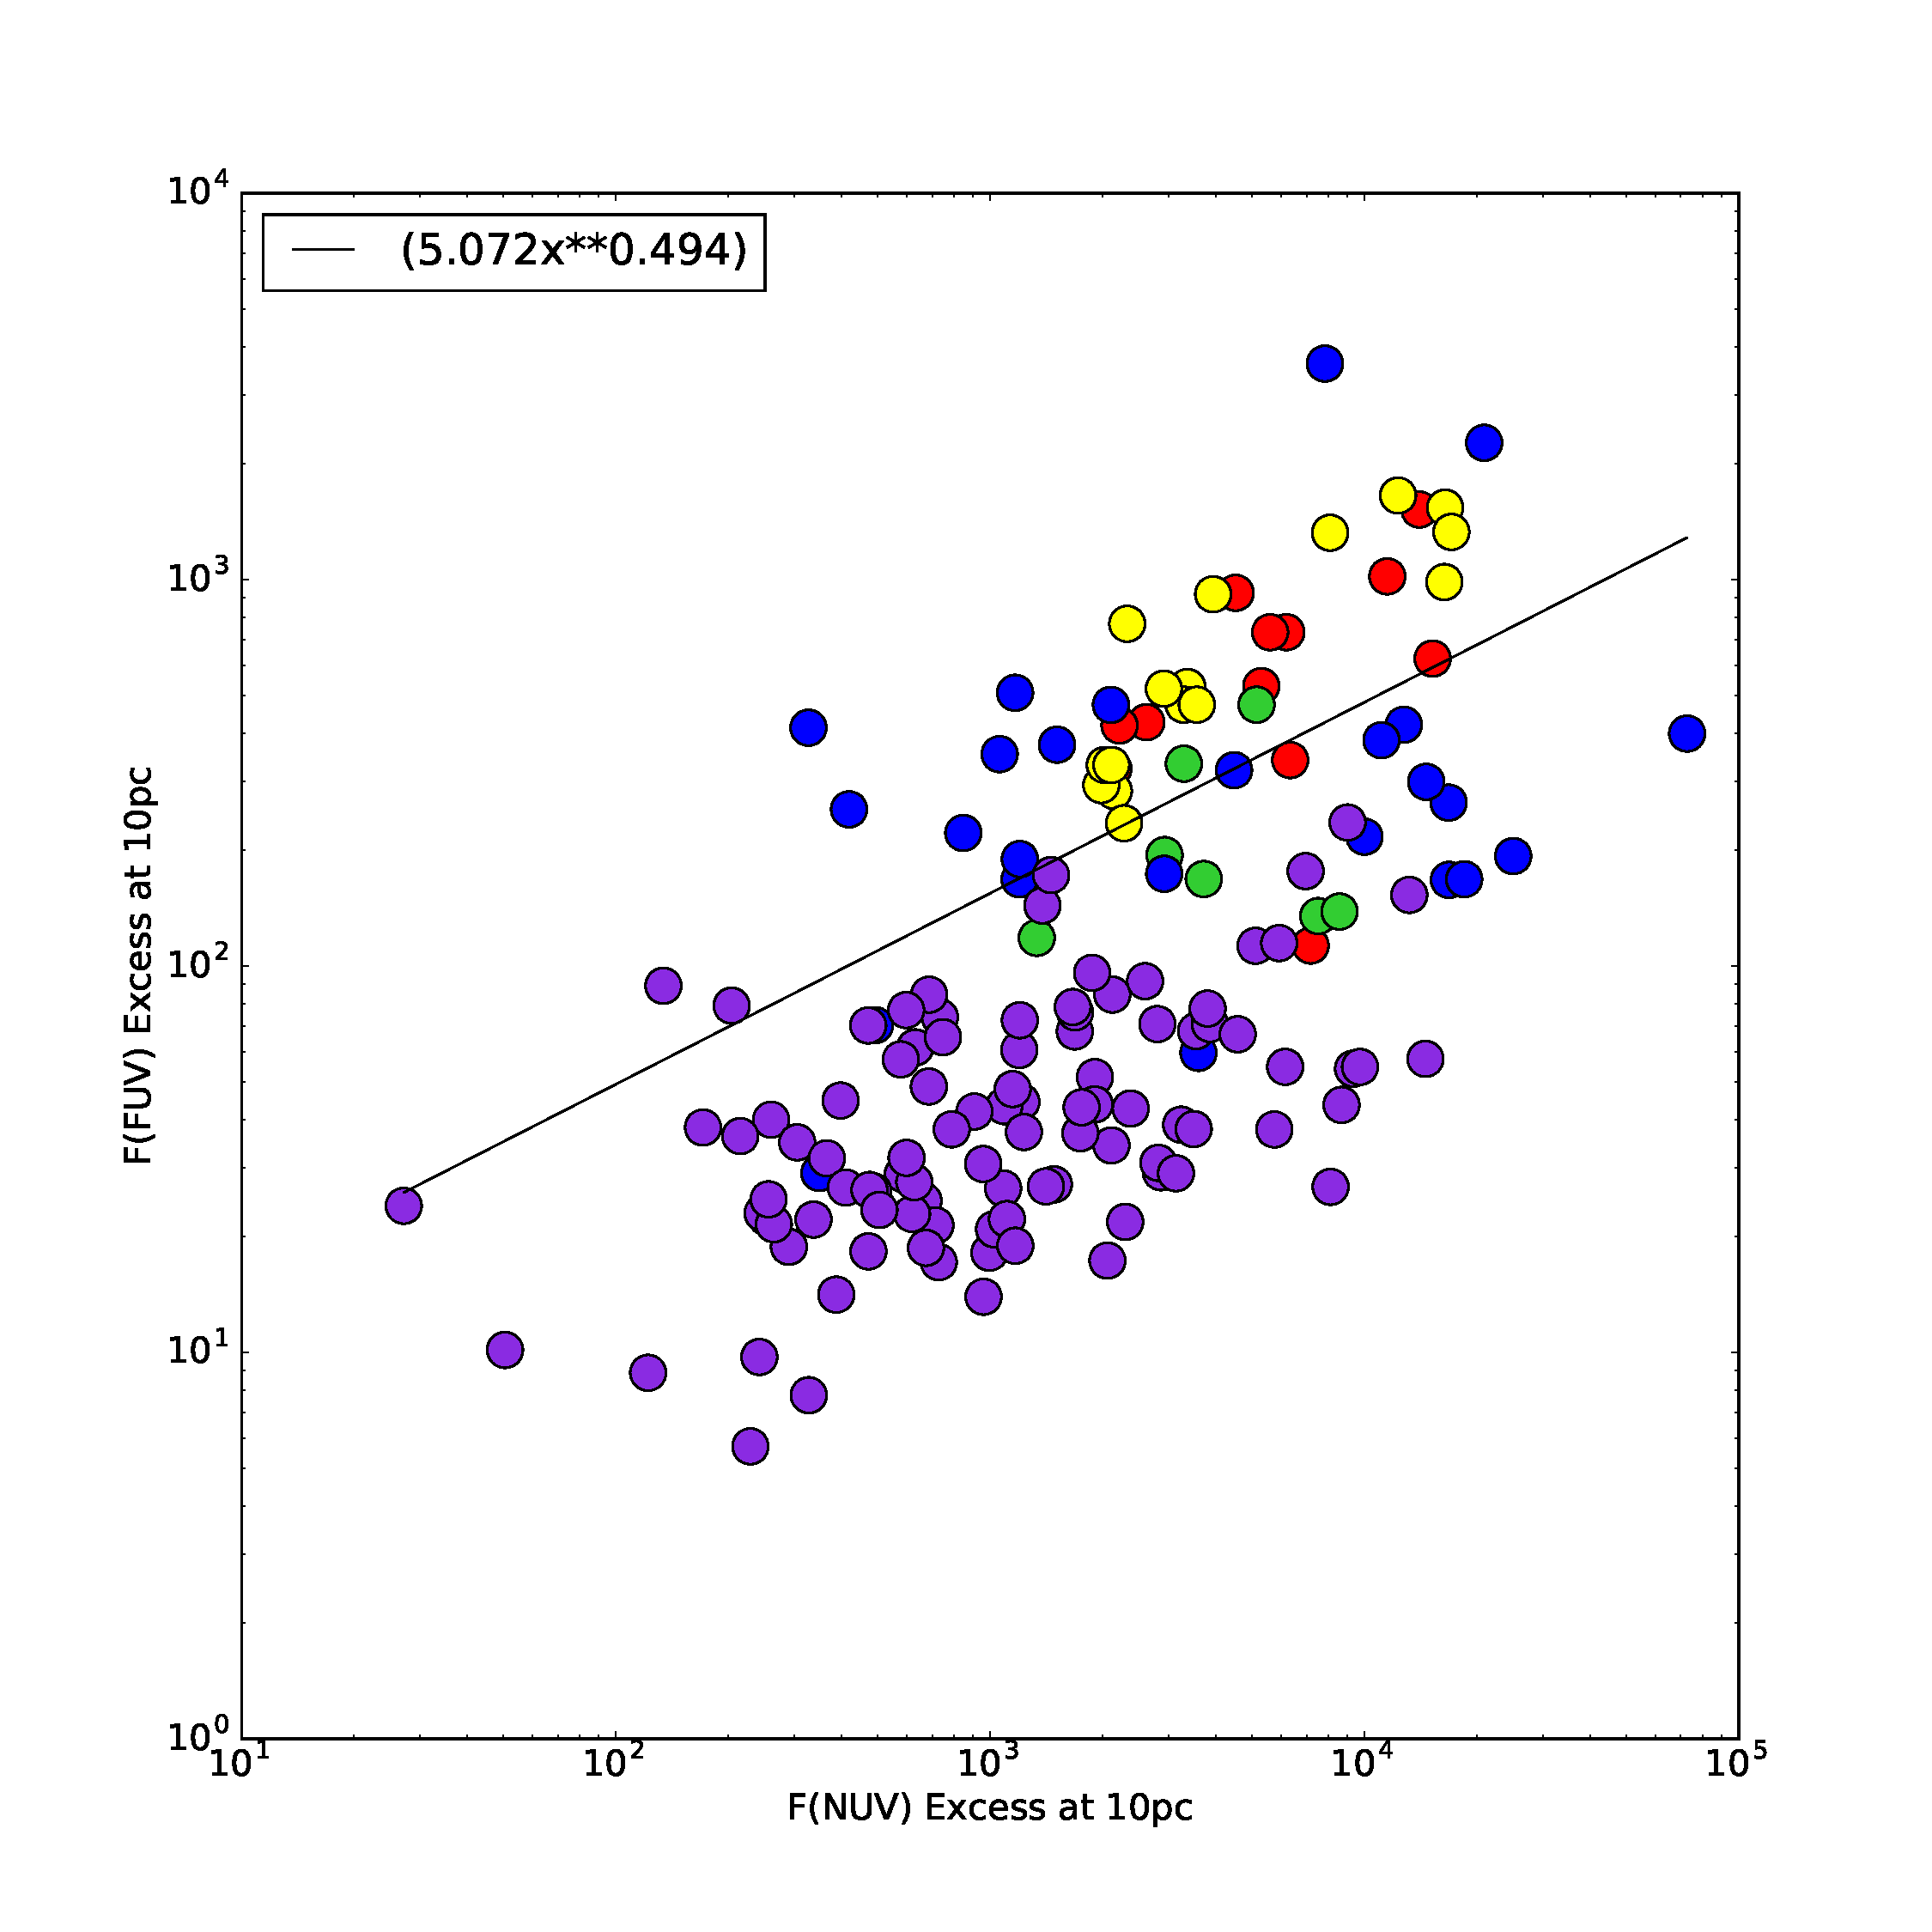
\includegraphics[width=\linewidth]{nuv_vs_fuv_NO_J.pdf}
\caption{Filler image for now. Need to fix scaling. \label{fig:nuv_vs_fuv}}
\end{figure*}

\begin{figure*}[h]
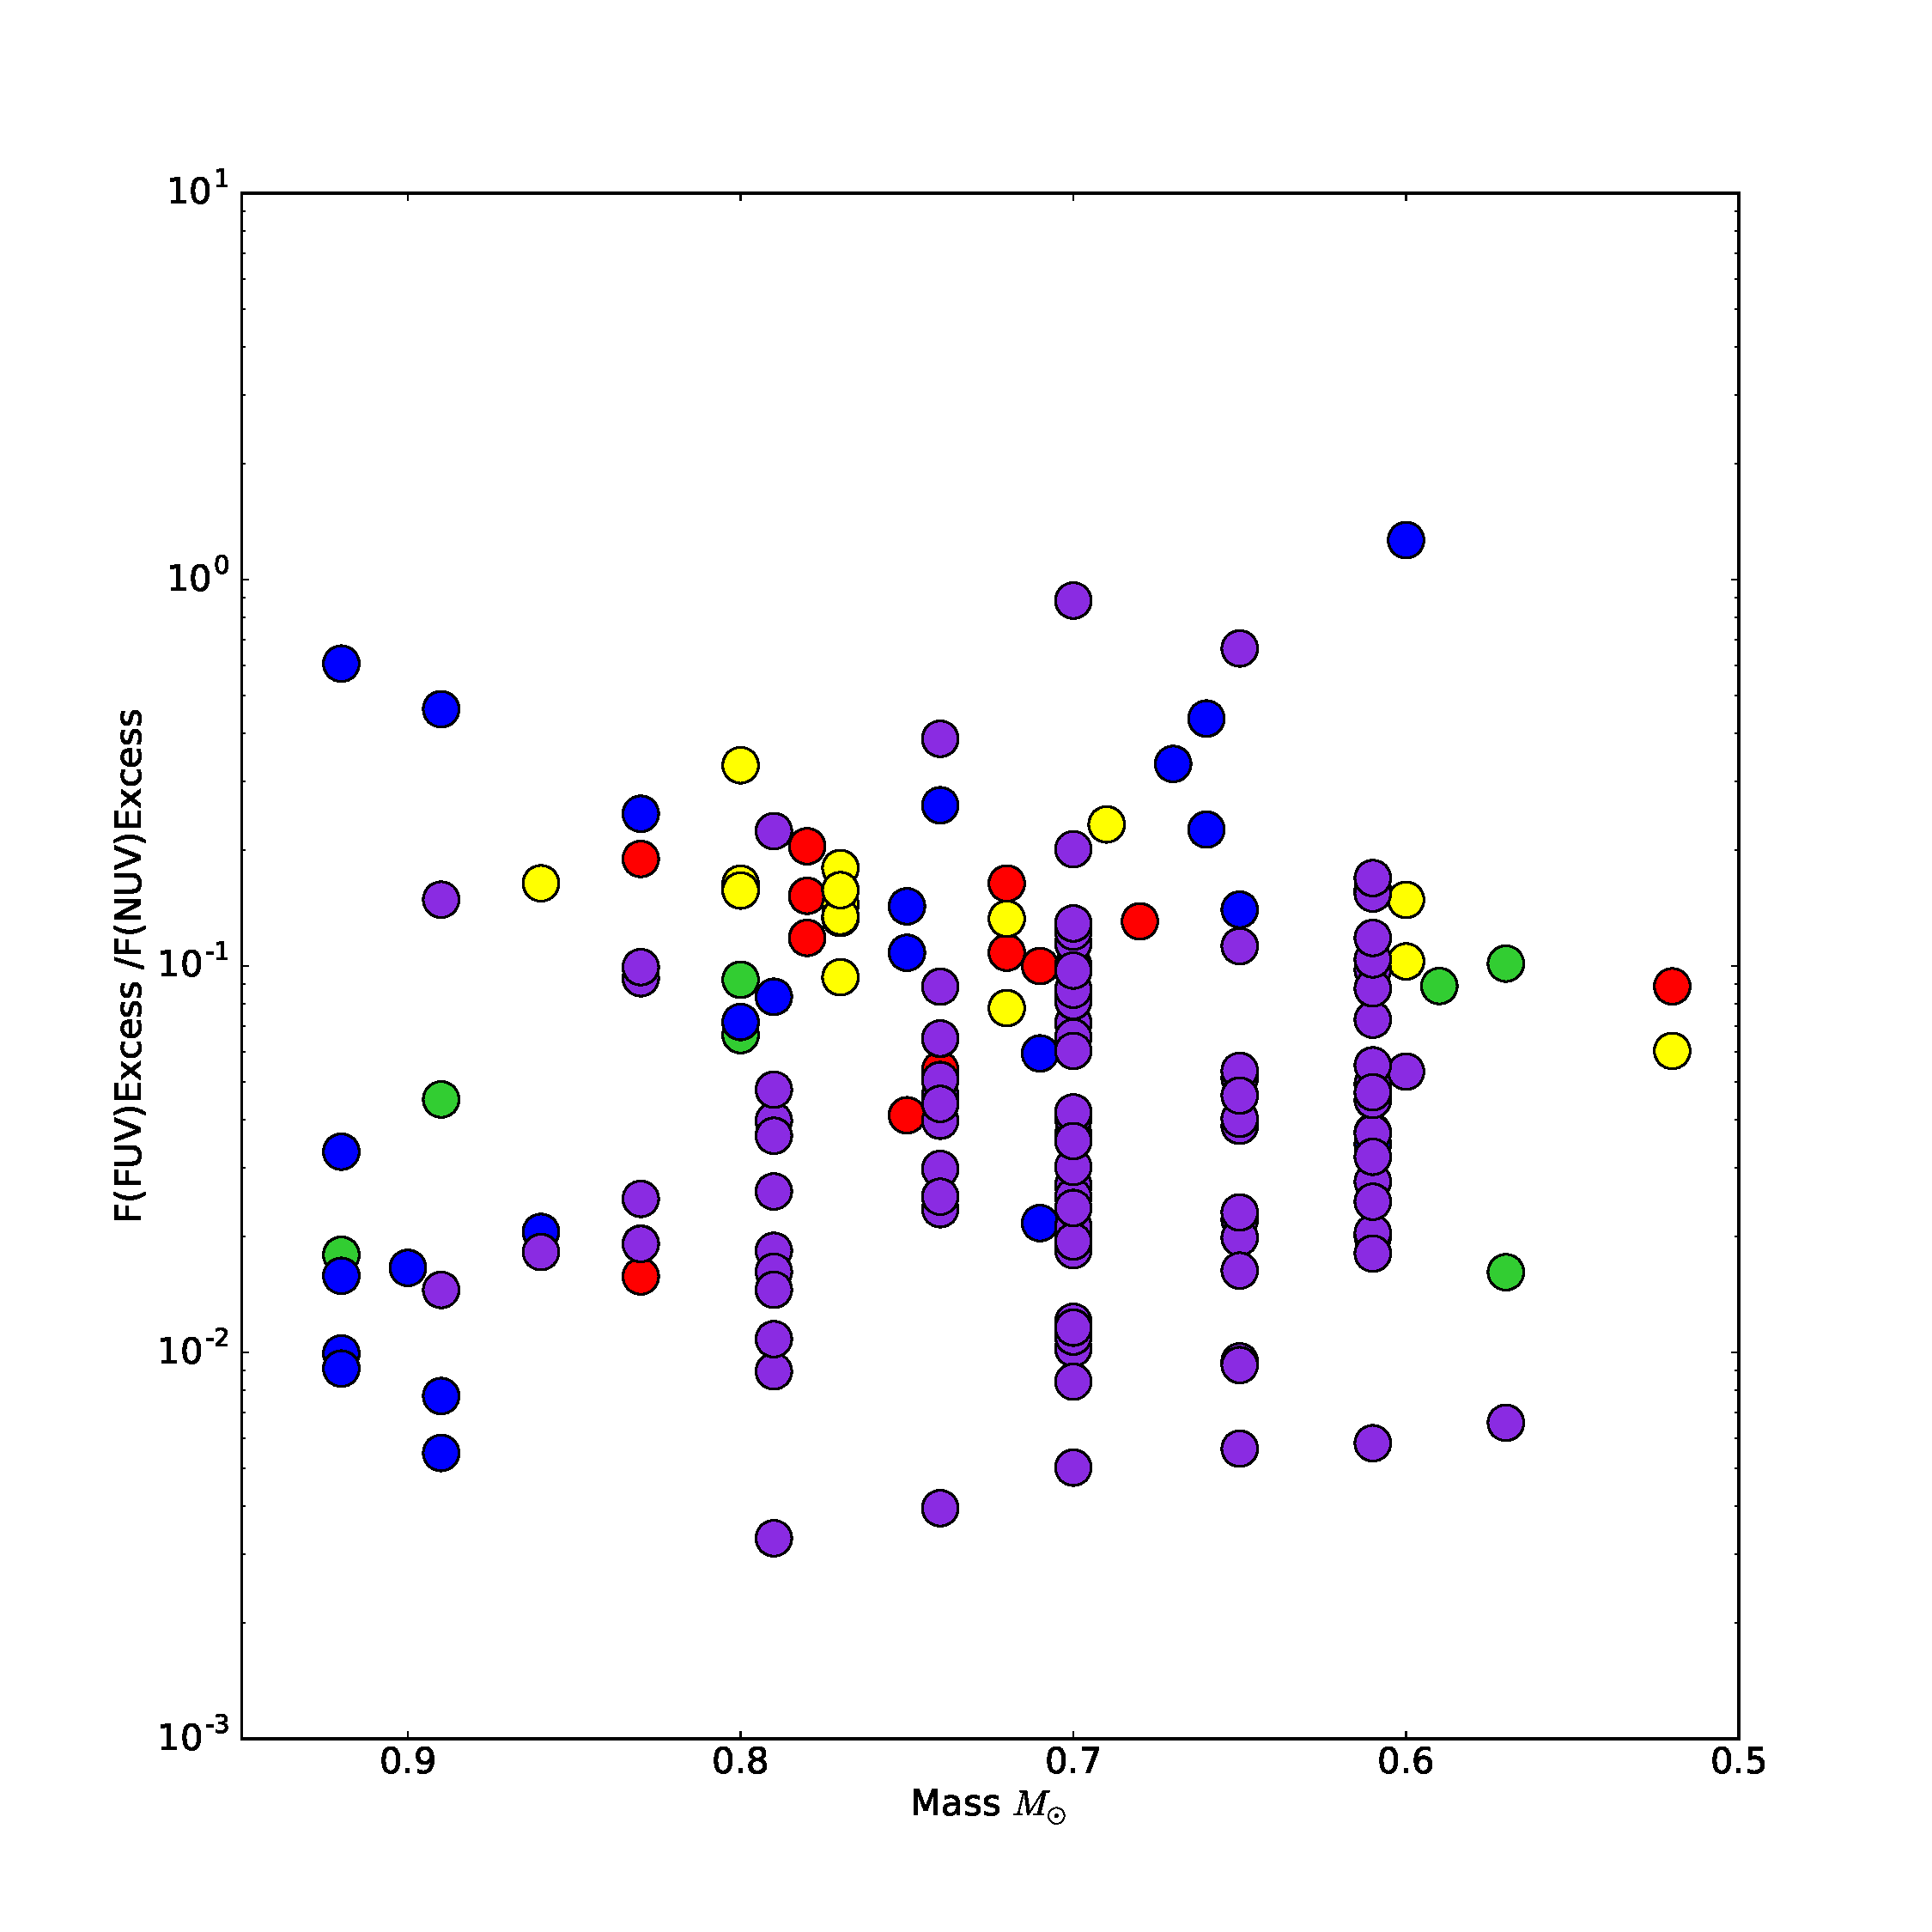
\includegraphics[width=\linewidth]{fuv_nuv_vs_mass_NO_J.pdf}
\caption{Filler image for now. Need to fix scaling. \label{fig:fuv_nuv_vs_mass}}
\end{figure*}

\subsubsection{Scatter}

\begin{figure*}[h]
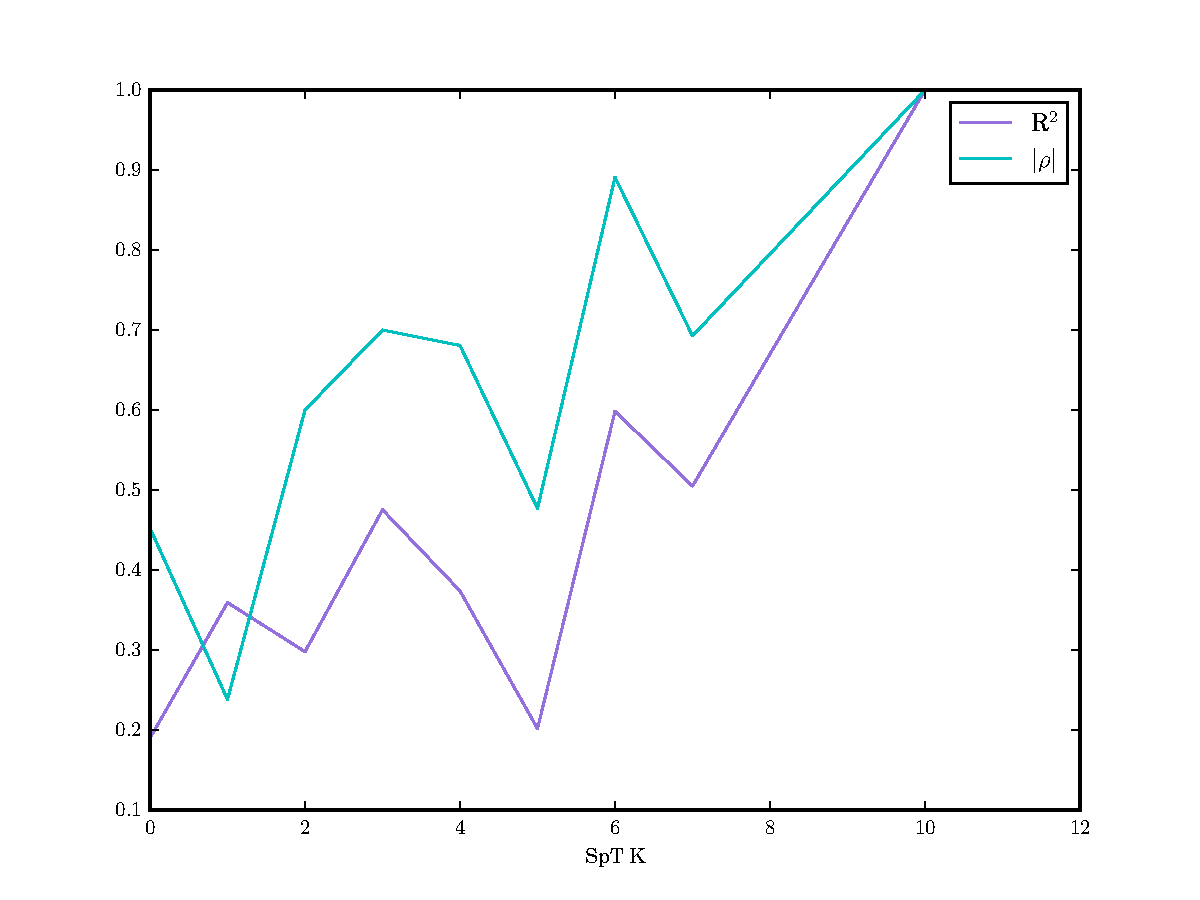
\includegraphics[width=\linewidth]{R2_vs_spt.pdf}
\caption{Filler image for now. Need to fix scaling. \label{fig:r2_vs_spt}}
\end{figure*}

\section{X-Ray Evolution}

\begin{figure*}[h]
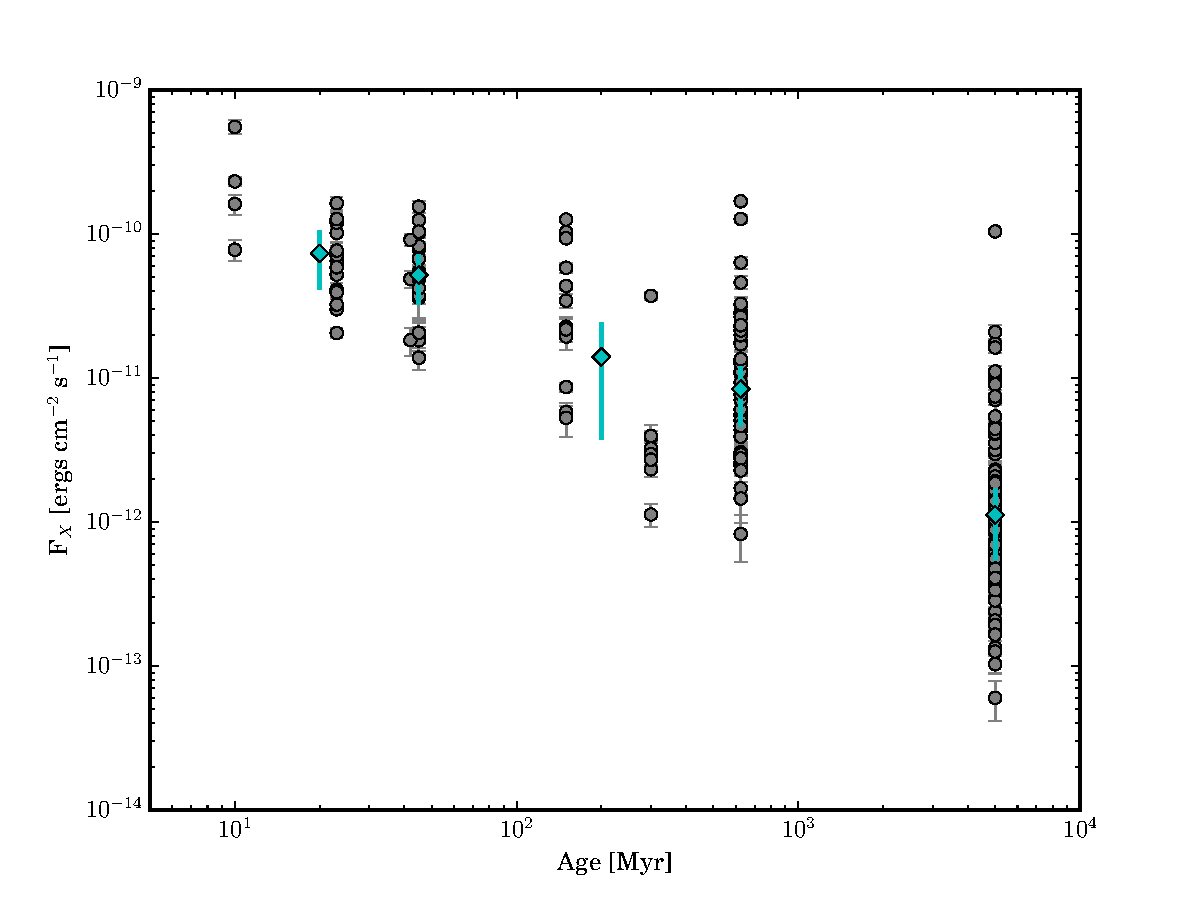
\includegraphics[width=\linewidth]{xray_evolution.pdf}
\caption{Filler image for now. Need to fix scaling. \label{fig:xray_evolution}}
\end{figure*}

\begin{figure*}[h]
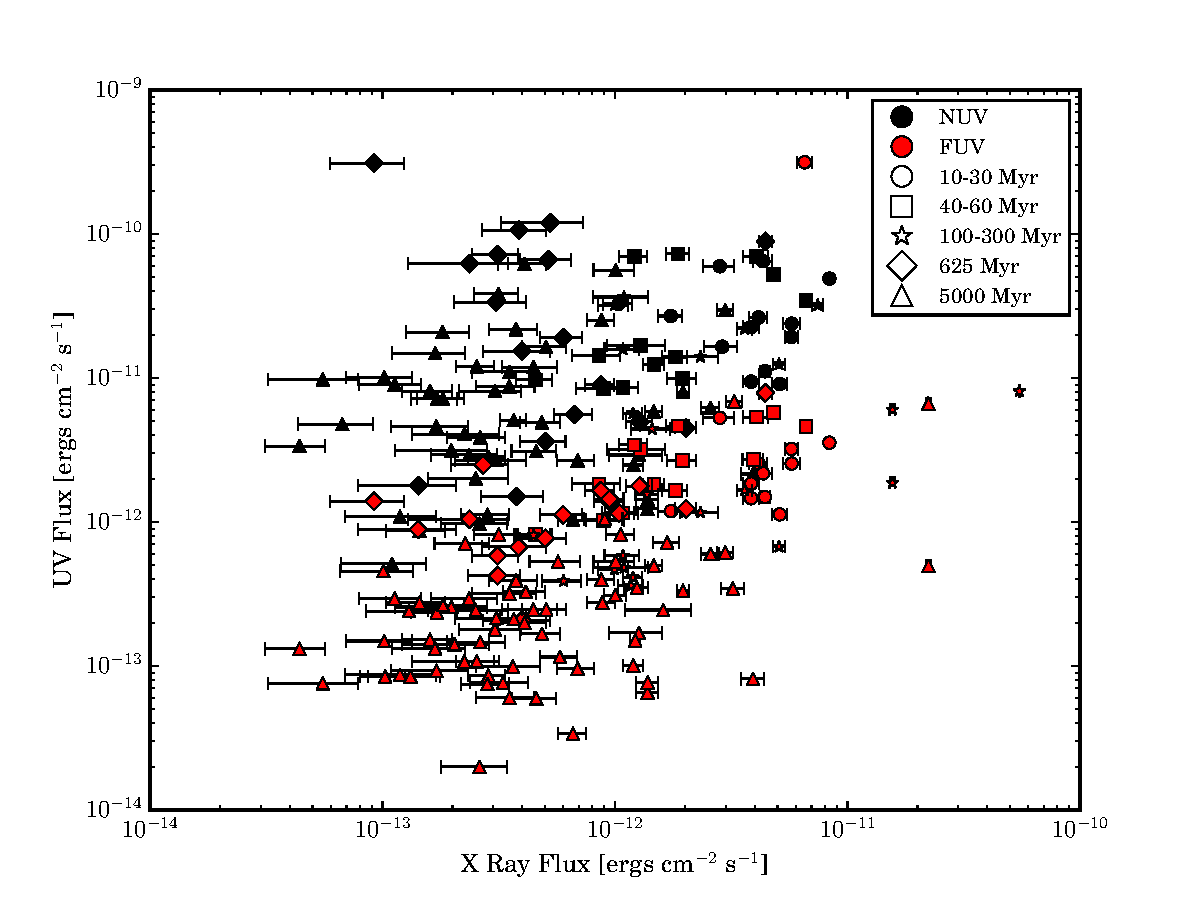
\includegraphics[width=\linewidth]{uv_vs_xray_NO_J.pdf}
\caption{Filler image for now. Need to fix scaling. \label{fig:uv_vs_xray}}
\end{figure*}

\begin{figure*}[h]
\centering
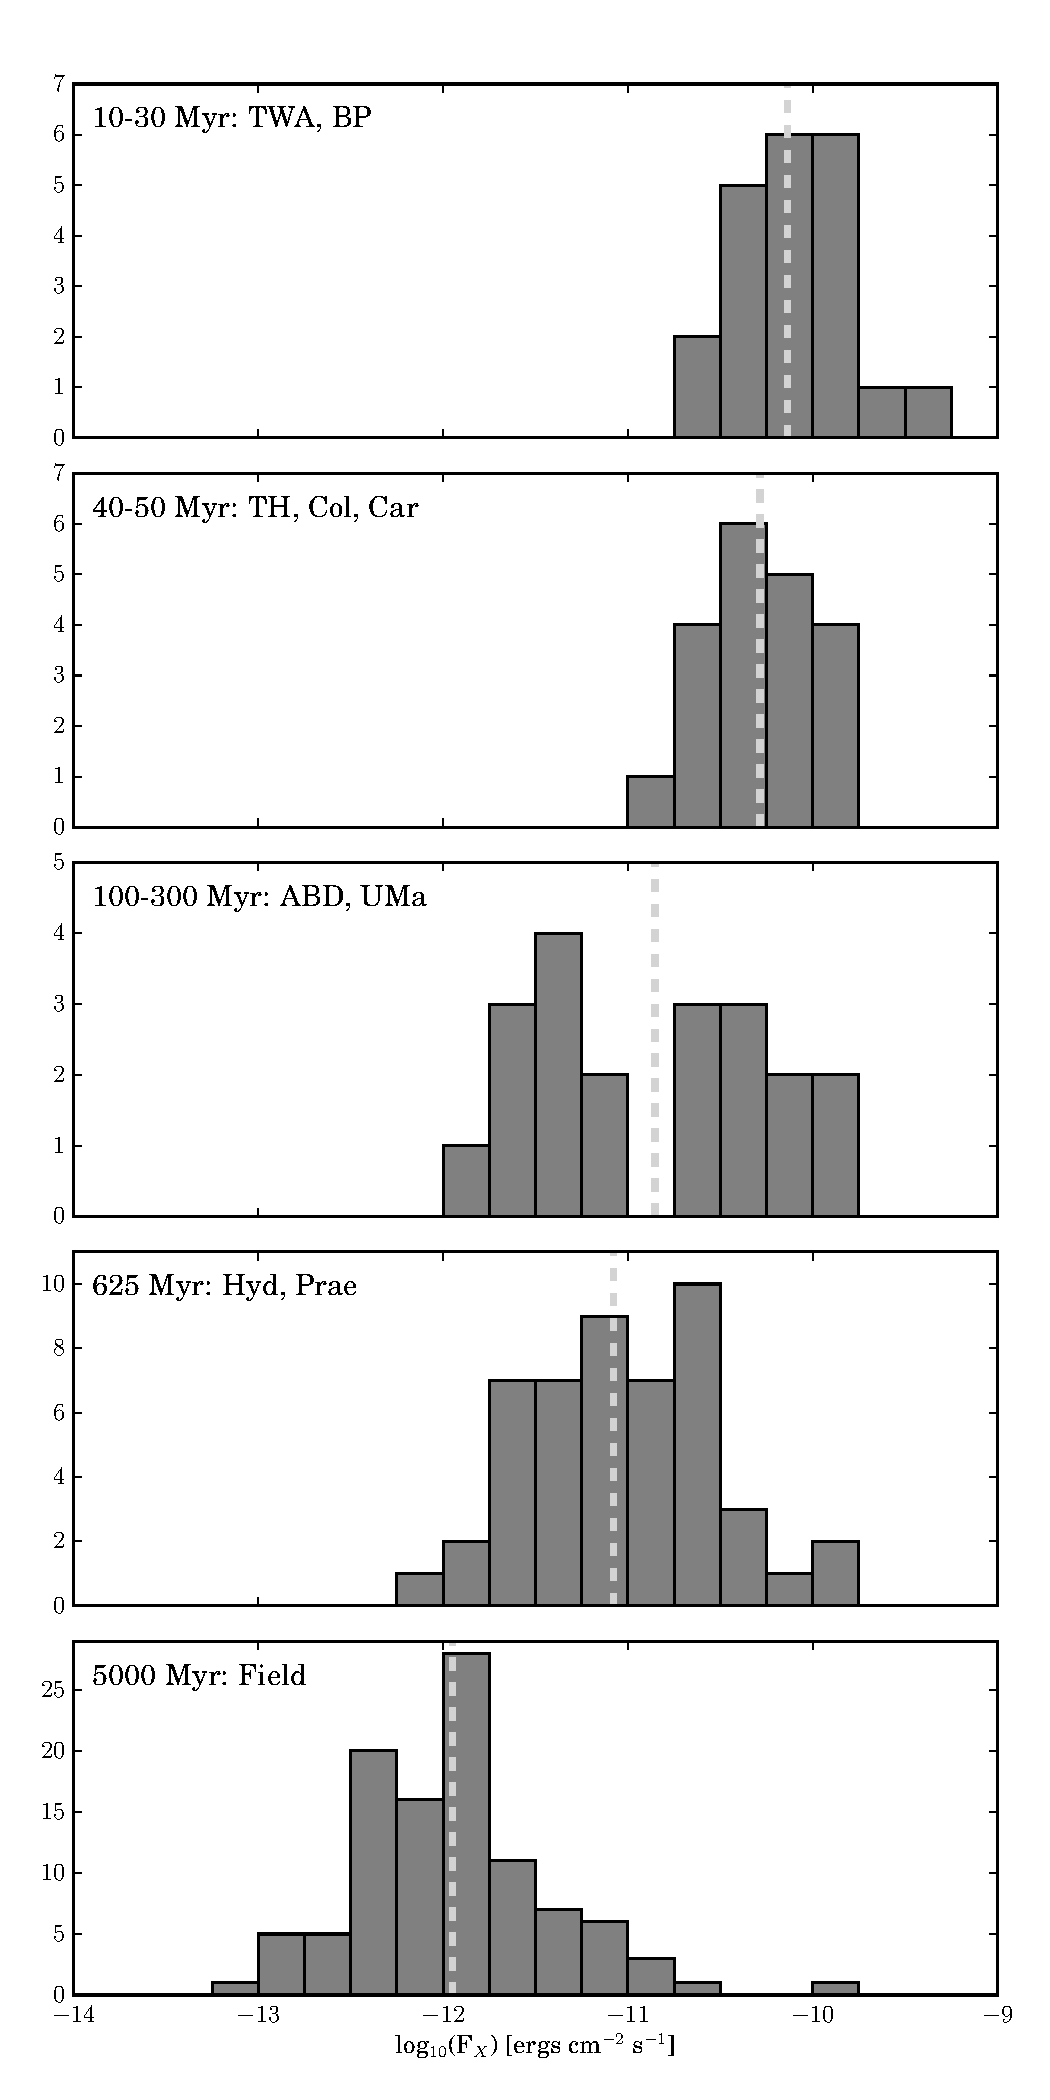
\includegraphics[height=\textheight]{histfd_xray.pdf}
\caption{Filler image for now. Need to fix scaling. \label{fig:histfd_xray}}
\end{figure*}

\section{Summary}

\begin{figure*}[h]
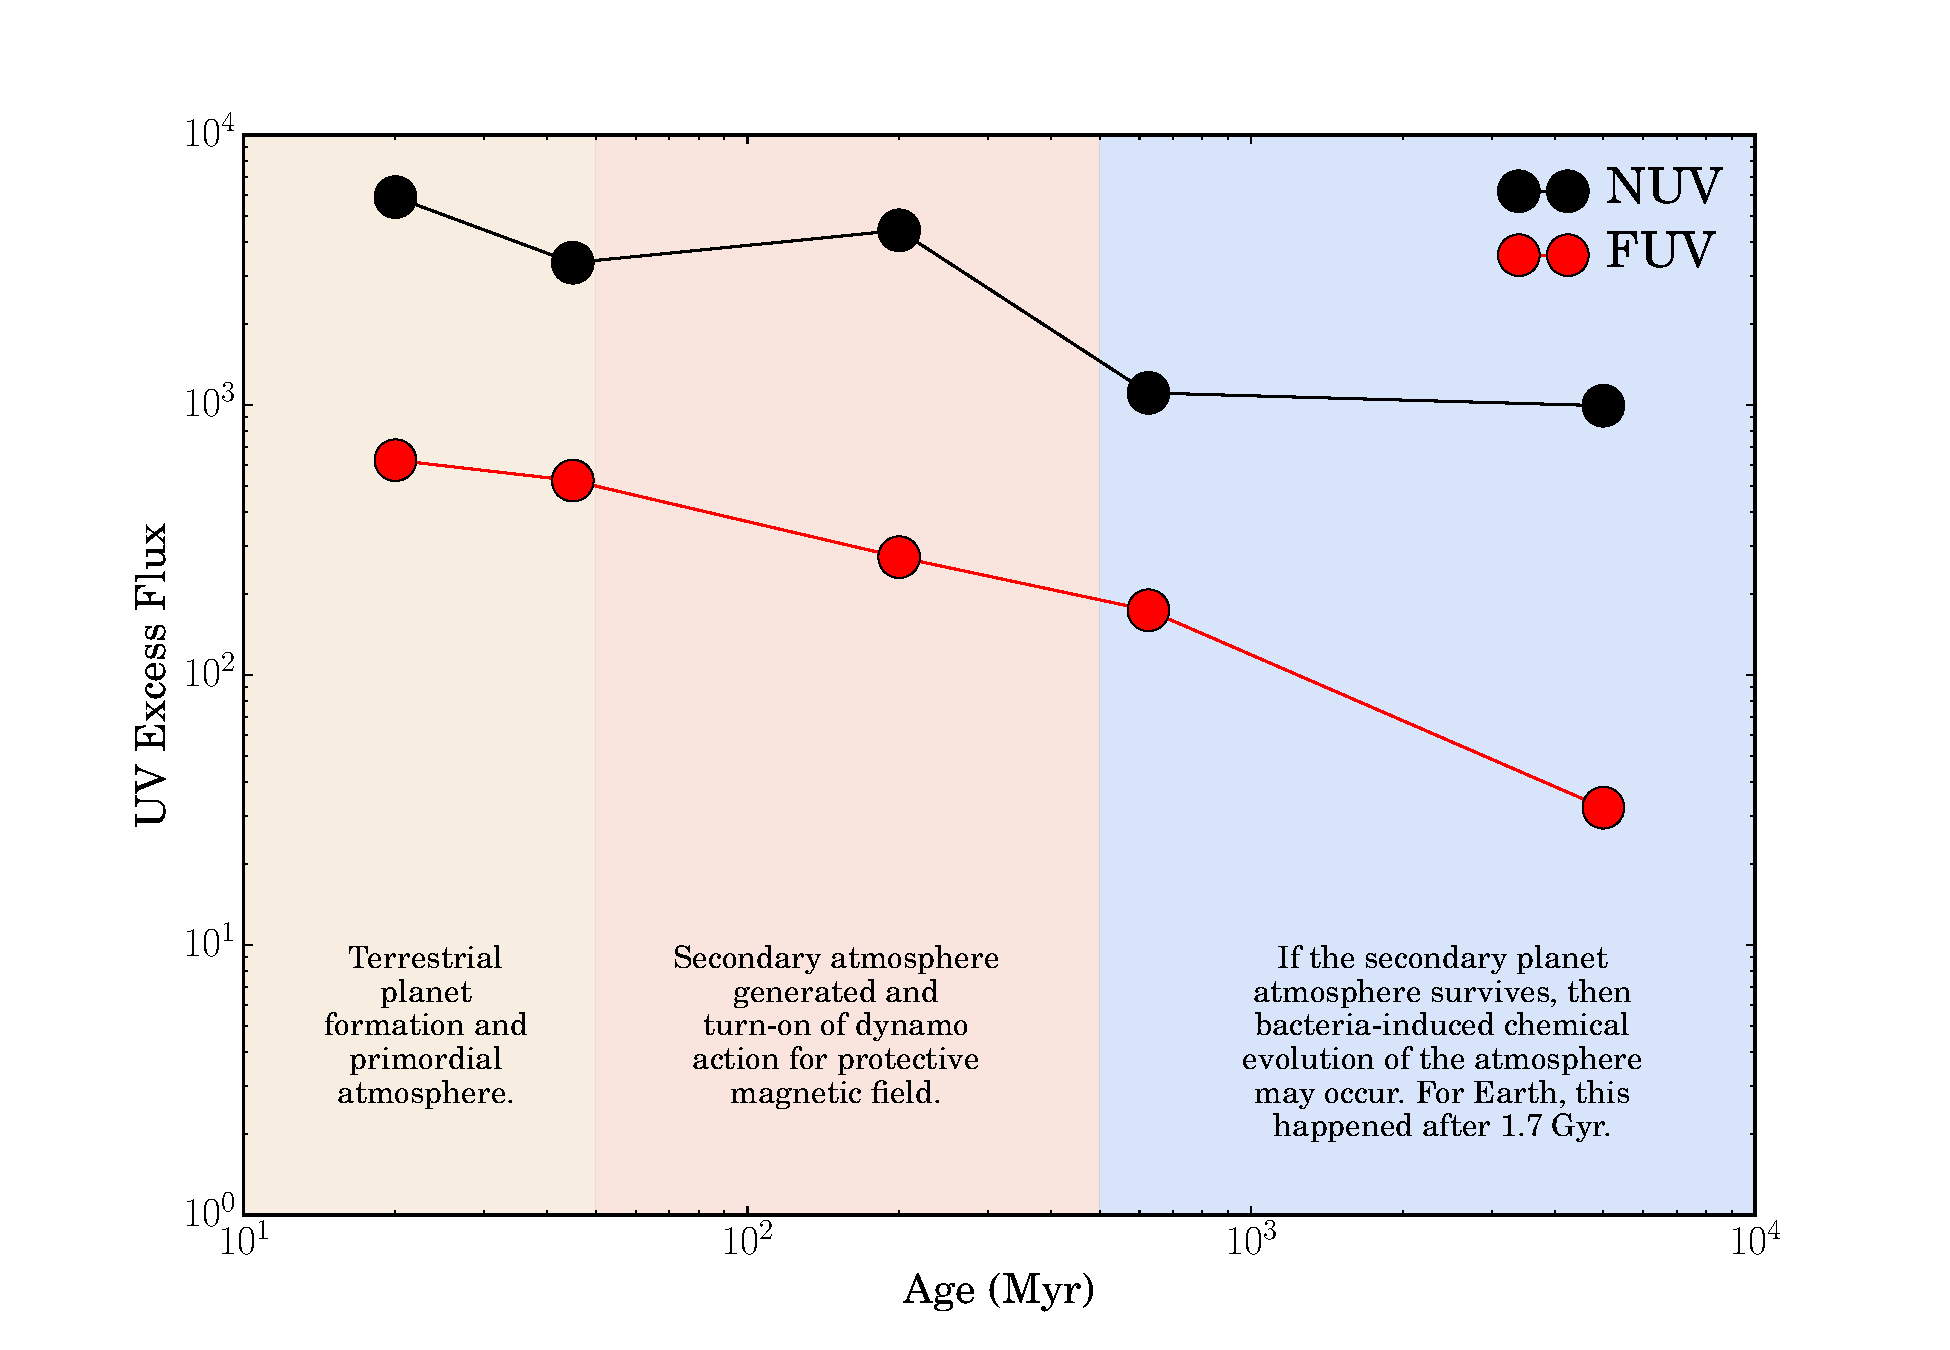
\includegraphics[width=\linewidth]{planet_timeline_NO_J.pdf}
\caption{Filler image for now. Need to fix scaling. \label{fig:planet_timeline}}
\end{figure*}

\bibliography{bibliography}

\end{document}
